\documentclass[%
%%% PARA ESCOLHER O ESTILO TIRE O SIMBOLO %(COMENTÁRIO)
%SemVinculoColorido,
%SemFormatacaoCapitulo,
SemFolhaAprovacao,
%SemImagens,
%CitacaoNumerica, %% o padrão é citação tipo autor-data
%PublicacaoDissOuTese, %% (é também o "default") com ficha catal. e folha de aprovação em branco. Caso tenha lista de símbolos e lista de siglas e abreviaturas retirar os comentários dos arquivos siglas.tex e abreviaturasesiglas.tex. Retirar também os comentários indicados nesse arquivo, nos includes
%PublicacaoArtigoOuRelatorio, %% texto sequencial, sem quebra de páginas nem folhas em branco
PublicacaoProposta, %% igual tese/dissertação, mas sem ficha catal. e fol. de aprov.
%PublicacaoLivro, %% com capítulos
%PublicacaoLivro,SemFormatacaoCapitulo, %% sem capítulos
english,portuguese %% para os documentos em Português com abstract.tex em Inglês
%portuguese,english %% para os documentos em Inglês com abstract.tex em Português
,LogoINPE% comentar essa linha para fazer aparecer o logo do Governo
,CCBYNC	% as opções de licença são: CCBY, CCBYSA, CCBYND, CCBYNC, CCBYNCSA, CCBYNCND, GPLv3 e INPECopyright
]{tdiinpe}
%]{../../../../../iconet.com.br/banon/2008/03.25.01.19/doc/tdiinpe}

% PARA EXIBIR EM ARIAL TIRAR O COMENTÁRIO DAS DUAS LINHAS SEGUINTES
%\renewcommand{\rmdefault}{phv} % Arial
%\renewcommand{\sfdefault}{phv} % Arial

% PARA PUBLICAÇÕES EM INGLÊS:
% renomear o arquivo: abnt-alf.bst para abnt-alfportuguese.bst
% renomear o arquivo: abnt-alfenglish.bst para abnt-alf.bst


%%%%%%%%%%%%%%%%%%%%%%%%%%%%%%%%%%%%%%%%%%%%%
%%% Pacotes já previamente carregados:      %
%%%%%%%%%%%%%%%%%%%%%%%%%%%%%%%%%%%%%%%%%%%%%%%%%%%%%%%%%%%%%%%%%%%%%%%%
%%% ifthen,calc,graphicx,color,inputenc,babel,hyphenat,array,setspace, %
%%% bigdelim,multirow,supertabular,tabularx,longtable,lastpage,lscape, %
%%% rotate,caption2,amsmath,amssymb,amsthm,subfigure,tocloft,makeidx,  %
%%% eso-pic,calligra,hyperref,ae,fontenc                               %
%%%%%%%%%%%%%%%%%%%%%%%%%%%%%%%%%%%%%%%%%%%%%%%%%%%%%%%%%%%%%%%%%%%%%%%%
%%% insira neste campo, comandos de LaTeX %%%
%%% \usepackage{_exemplo_}
% etc.
%%%%%%%%%%%%%%%%%%%%%%%%%%%%%%%%%%%%%%%%%%%%%

%\watermark{Revisão No. ##} %% use o comando \watermark para identificar a versão de seu documento
%% comente este comando quando for gerar a versão final
%\usepackage{subcaption}
\usepackage{adjustbox}
\usepackage{rotating}
\usepackage{hyperref}
\usepackage{float}
\usepackage{svg}
\usepackage{epstopdf}
\usepackage{rotating}
\usepackage{dsfont}
\usepackage{comment}
%%%%%%%%%%%%%%%%%%%CAPA%%%%%%%%%%%%%%%%%%%%%%%%%%%%%%%%
%\serieinpe{INPE-NNNNN-TDI/NNNN} %% n\~{a}o mais usado

\titulo{Escrever o t\'{i}tulo no idioma em que foi escrito a publicaç\~{a}o}
\title{Escrever o t\'{i}tulo em Ingl\^{e}s para publicaç\~{o}es escritas em Portugu\^{e}s e em Portugu\^{e}s para publicaç\~{o}es escritas em Ingl\^{e}s} %% 
\author{Nome Completo do Autor} %% coloque o nome do(s) autor(es)
\descriccao{Tese de Doutorado ou Dissertaç\~{a}o de Mestrado do Curso de P\'{o}s-Graduaç\~{a}o em Nome do Curso, orientada pelo(a) Dr(a). Nome do Orientador(a), aprovada em dd de m\^{e}s por extenso de aaaa.}
\repositorio{aa/bb/cc/dd} %% reposit\'{o}rio onde est\'{a} depositado este documento - na omiss\~{a}o, ser\'{a} preenchido pelo SID
\tipoDaPublicacao{TDI}	%% tipo da publicaç\~{a}o (NTC, RPQ, PRP, MAN, PUD, TDI, TAE e PRE) na aus\^{e}ncia do n\'{u}mero de s\'{e}rie INPE, caso contr\'{a}rio deixar vazio
\IBI{xx/yy} %% IBI (exemplo: J8LNKAN8PW/36CT2G2) quando existir, caso contr\'{a}rio o nome do reposit\'{o}rio onde est\'{a} depositado o documento

\date{AAAA}%ano da publicaç\~{a}o

%%%%%%%%%%%%%%%%%%%%%%%%%%VERSO DA CAPA%%%%%%%%%%%%%%%%%%%%%%%%%%%%%%%%%%%%%%%%%%%%%%%
\tituloverso{\vspace{-0.9cm}\textbf{\PublicadoPor:}}
\descriccaoverso{Instituto Nacional de Pesquisas Espaciais - INPE\\
Gabinete do Diretor (GB)\\
Serviço de Informaç\~{a}o e Documentaç\~{a}o (SID)\\
Caixa Postal 515 - CEP 12.245-970\\
S\~{a}o Jos\'{e} dos Campos - SP - Brasil\\
Tel.:(012) 3945-6923/6921\\
Fax: (012) 3945-6919\\
E-mail: {\url{pubtc@sid.inpe.br}}
}

\descriccaoversoA{\textbf{\ConselhoDeEditoracao:}\\
\textbf{\Presidente:}\\
Marciana Leite Ribeiro - Serviço de Informaç\~{a}o e Documentaç\~{a}o (SID)\\
\textbf{\Membros:}\\
Dr. Gerald Jean Francis Banon - Coordenaç\~{a}o Observaç\~{a}o da Terra (OBT)\\
Dr. Amauri Silva Montes - Coordenaç\~{a}o Engenharia e Tecnologia Espaciais (ETE)\\
Dr. Andr\'{e} de Castro Milone - Coordenaç\~{a}o Ci\^{e}ncias Espaciais e Atmosf\'{e}ricas (CEA)\\
Dr. Joaquim Jos\'{e} Barroso de Castro -  Centro de Tecnologias Espaciais (CTE)\\
Dr. Manoel Alonso Gan - Centro de Previs\~{a}o de Tempo e Estudos Clim\'{a}ticos (CPT)\\
Drª Maria do Carmo de Andrade Nono - Conselho de P\'{o}s-Graduaç\~{a}o\\
Dr. Pl\'{i}nio Carlos Alval\'{a} - Centro de Ci\^{e}ncia do Sistema Terrestre (CST)\\
\textbf{\BibliotecaDigital:}\\
Dr. Gerald Jean Francis Banon - Coordenaç\~{a}o de Observaç\~{a}o da Terra (OBT)\\
Clayton Martins Pereira - Serviço de Informaç\~{a}o e Documentaç\~{a}o (SID)\\
%Jefferson Andrade Ancelmo - Serviço de Informaç\~{a}o e Documentaç\~{a}o (SID)\\
%Simone A. Del-Ducca Barbedo - Serviço de Informaç\~{a}o e Documentaç\~{a}o (SID)\\
%Deicy Farabello - Centro de Previs\~{a}o de Tempo  e Estudos Clim\'{a}ticos (CPT)\\
\textbf{\RevisaoNormalizacaoDocumentaria:}\\
Simone Ang\'{e}lica Del Ducca Barbedo - Serviço de Informaç\~{a}o e Documentaç\~{a}o (SID) \\
%Maril\'{u}cia Santos Melo Cid - Serviço de Informaç\~{a}o e Documentaç\~{a}o (SID)\\
Yolanda Ribeiro da Silva Souza - Serviço de Informaç\~{a}o e Documentaç\~{a}o (SID)\\
\textbf{\EditoracaoEletronica:}\\
Marcelo de Castro Pazos - Serviço de Informaç\~{a}o e Documentaç\~{a}o (SID)\\
Andr\'{e} Luis Dias Fernandes - Serviço de Informaç\~{a}o e Documentaç\~{a}o (SID)\\
}

%%%%%%%%%%%%%%%%%%%FOLHA DE ROSTO

%%%%%%%%%%%%%%%FICHA CATALOGRÁFICA
%% NÃO PREENCHER - SERÁ PREENCHIDO PELO SID

\cutterFICHAC{Cutter}
\autorUltimoNomeFICHAC{Sobrenome, Nomes} %% exemplo: Fuckner, Marcus Andr\'{e}
\autorAbreviadoFICHAC {} %% N\~{a}o usado - deixar vazio
\tituloFICHAC{Titulo da publicaç\~{a}o}
\instituicaosigla{INPE}
\instituicaocidade{S\~{a}o Jos\'{e} dos Campos}
\paginasFICHAC{\pageref{numeroDePaginasDoPretexto} + \pageref{LastPage}} %% n\'{u}mero total de p\'{a}ginas
%\serieinpe{INPE-00000-TDI/0000} %% n\~{a}o mais usado
\palavraschaveFICHAC{1.~Palavra chave. 2.~Palavra chave 3.~Palavra chave. 4.~Palavra chave. 5.~Palavra chave  I.~\mbox{T\'{i}tulo}.} %% recomenda-se pelo menos 5 palavras-chaves - \mbox{} \'{e} para evitar hifenizaç\~{a}o 
\numeroCDUFICHAC{000.000} %% n\'{u}mero do CDU 

% Nota da ficha (para TD)
\tipoTD{Dissertaç\~{a}o ou Tese} % Dissertaç\~{a}o ou Tese
\cursoFA{Mestrado ou Doutorado em Nome do Curso}
\instituicaoDefesa{Instituto Nacional de Pesquisas Espaciais}
\anoDefesa{AAAA} % ano de defesa 
\nomeAtributoOrientadorFICHAC{Orientador}	% pode ser: Orientador, Orientadora ou Orientadores
\valorAtributoOrientadorFICHAC{Jos\'{e} da Silva} % nome(s) completo(s)

%%%%%%%%%%%%%%%FOLHA DE APROVAÇAO PELA BANCA EXAMINADORA
\tituloFA{\textbf{ATENÇÃO! A FOLHA DE APROVAÇÃO SERÁ INCLUIDA POSTERIORMENTE.}}
%\cursoFA{\textbf{}}
\candidatoOUcandidataFA{}
\dataAprovacaoFA{}
\membroA{}{}{}
\membroB{}{}{}
\membroC{}{}{}
\membroD{}{}{}
\membroE{}{}{}
\membroF{}{}{}
\membroG{}{}{}
\ifpdf

%%%%%%%%%%%%%%NÍVEL DE COMPRESSÃO {0 -- 9}
\pdfcompresslevel 9
\fi
%%% define em 80% a largura das figuras %%%
\newlength{\mylenfig} 
\setlength{\mylenfig}{0.8\textwidth}
%%%%%%%%%%%%%%%%%%%%%%%%%%%%%%%%%%%%%%%%%%%

%%%%%%%%%%%%%%COMANDOS PESSOAIS
\newcommand{\vetor}[1]{\mathit{\mathbf{#1}}} %% faça as modificações pertinentes no arquivo configuracao.tex

\makeindex  %% não alterar, gera INDEX, caso haja algum termo indexado no texto

\begin{document} %% início do documento %% não mexer

%\marcaRegistrada{}	% comando opcional usado para informar abaixo da ficha catalográfica sobre marca registrada
\marcaRegistrada{Informar aqui sobre marca registrada (a modificação desta linha deve ser feita no arquivo publicacao.tex).}

\maketitle  %% não alterar, gera páginas obrigatórias (folha de rosto, ficha catalográfica e folha de aprovação), automaticamente

%%% Comente as linhas opcionais abaixo caso não as deseje
%%%%%%%%%%%%%%%%%%%%%%%%%%%%%%%%%%%%%%%%%%%%%%%%%%%%%%%%%%%%%%%%%%%%%%%%%%%%%%%%%
% Epígrafe %% opcional

\begin{epigrafe} %% insira sua epígrafe abaixo; estilo livre

\hypertarget{estilo:epigrafe}{} %% uso para este Guia
 
\textit{\large``A vida será mais complicada se você possuir uma curiosidade ativa, além de aumentarem as chances de você entrar em apuros, mas será mais divertida''.}

\vspace{1cm}

\hspace{4cm} \emph{\textsc{Edward Speyer}}\\\hspace{4cm} em \textsl{``Seis Caminhos a Partir de Newton''}, 1994

\end{epigrafe}
 %% Opcional
%%%%%%%%%%%%%%%%%%%%%%%%%%%%%%%%%%%%%%%%%%%%%%%%%%%%%%%%%%%%%%%%%%%%%%%%%%%%%%%%%
% Dedicatória %% opcional

\begin{dedicatoria} %% insira sua dedicatória abaixo; estilo livre

\hypertarget{estilo:dedicatoria}{} %% uso para este Guia
 
%% use 'a meus' em vez de 'aos meus', isto é, não use o artigo definido com pronomes possessivos

\newcommand{\mytext}{A meus pais \textbf{Nicanor} e \textbf{Jaci}, à minha irmã \textbf{Luciana} e ao meu esposo \textbf{William}}

\begin{comment}
%%% sugestão de estilo
\ifcalligra %% fonte calligra presente nas versões mais novas do MiKTeX (>= 2.4)
  \calligra\Large \mytext %% exemplo usando estilo de fonte caligráfica, caso haja
\else
	\itshape\Large \mytext 
\fi
\end{comment}

	\itshape\Large \mytext 

\end{dedicatoria} %% Opcional
%%%%%%%%%%%%%%%%%%%%%%%%%%%%%%%%%%%%%%%%%%%%%%%%%%%%%%%%%%%%%%%%%%%%%%%%%%%%%%%%%
% AGRADECIMENTOS %% opcional

\begin{agradecimentos}  %% insira abaixo seus agradecimentos

\hypertarget{estilo:agradecimentos}{} %% uso para este Guia
Agradecemos à MsC Andriana Susana Lopes de Oliveira Campanharo que gentilmente cedeu 
parte dos textos de sua dissertação para este estilo. O original de sua dissertação
encontra-se na Biblioteca Digital do INPE, no endereço \url {http://urlib.net/sid.inpe.br/MTC-m13@80/2006/11.07.12.37}.
Agradecemos também ao Dr. Gerald Jean Francis Banon pelo desenvolvimento e disponibilização deste estilo.
\end{agradecimentos}


 %% Opcional
%%%%%%%%%%%%%%%%%%%%%%%%%%%%%%%%%%%%%%%%%%%%%%%%%%%%%%%%%%%%%%%%%%%%%%%%%%%%%%%%%
% RESUMO %% obrigatório

\begin{resumo}

%% neste arquivo resumo.tex
%% o texto do resumo e as palavras-chave têm que ser em Português para os documentos escritos em Português
%% o texto do resumo e as palavras-chave têm que ser em Inglês para os documentos escritos em Inglês
%% os nomes dos comandos \begin{resumo}, \end{resumo}, \palavraschave e \palavrachave não devem ser alterados

\hypertarget{estilo:resumo}{} %% uso para este Guia

Neste trabalho é analisada a possível natureza caótica da turbulência atmosférica. As análises aqui realizadas, baseadas em dados de temperatura de alta resolução, obtidos pela campanha WETAMC do projeto LBA, sugerem a existência de um comportamento caótico de baixa dimensão na camada limite atmosférica. O atrator caótico correspondente possui uma dimensão de correlação de $D_{2}=3.50\pm0.05$. A presença de dinâmica caótica nos dados analisados é confirmada com a estimativa de um expoente de Lyapunov pequeno mas positivo, com valor $\lambda_{1}=0.050\pm0.002$. No entanto, esta dinâmica caótica de baixa dimensão está associada à presença das estruturas coerentes na camada limite atmosférica e não à turbulência atmosférica. Esta afirmação é evidenciada pelo processo de filtragem por wavelets utilizado nos dados experimentais estudados, que permite separar a contribuição da estruturas coerentes do sinal turbulento de fundo.

\palavraschave{%
	\palavrachave{Turbulência atmosférica}%
	\palavrachave{Campanha WETAMC}%
	\palavrachave{Projeto LBA}%
	\palavrachave{Comportamento caótico}%
	\palavrachave{Atrator caótico}%
}
 
\end{resumo} %% obrigatório
%%%%%%%%%%%%%%%%%%%%%%%%%%%%%%%%%%%%%%%%%%%%%%%%%%%%%%%%%%%%%%%%%%%%%%%%%%%%%%%%%
% ABSTRACT


\begin{abstract}

%% neste arquivo abstract.tex
%% o texto do resumo e as palavras-chave têm que ser em Inglês para os documentos escritos em Português
%% o texto do resumo e as palavras-chave têm que ser em Português para os documentos escritos em Inglês
%% os nomes dos comandos \begin{abstract}, \end{abstract}, \keywords e \palavrachave não devem ser alterados

\selectlanguage{english}	%% para os documentos escritos em Português
%\selectlanguage{portuguese}	%% para os documentos escritos em Inglês

\hypertarget{estilo:abstract}{} %% uso para este Guia

In this work the possible chaotic nature of the atmospheric turbulence is analysed. The analyses carried out here, based in data of high resolution temperature, obtained from the WETAMC campaign of the LBA project, suggest the existence of a low-dimension chaotic behavior in the atmospheric boundary layer. The corresponding chaotic attractor possess a correlation dimension of $D_{2}=3.50\pm0.05$. The presence of chaotic dynamics in the analysed data is confirmed with the estimate of a small Lyapunov exponent but positive, with value $\lambda_{1}=0.050\pm0.002$. However, this low-dimension chaotic dynamics is associated with the presence of the coherent structures in the atmospheric boundary layer and not to the atmospheric turbulence. This affirmation is evidenced by the process of filtering for wavelets used in the studied experimental data, that allow to separate the contribution of the coherent structures of the turbulent background signal. 

\keywords{%
	\palavrachave{Atmospheric turbulence}%
	\palavrachave{WETAMC campaign}%
	\palavrachave{LBA project}%
	\palavrachave{Chaotic behavior}%
	\palavrachave{Chaotic attractor}%
}

\selectlanguage{portuguese}	%% para os documentos escritos em Português
%\selectlanguage{english}	%% para os documentos escritos em Inglês

\end{abstract} %% obrigatório

\includeListaFiguras %% obrigatório caso haja mais de 3 figuras, gerado automaticamente
\includeListaTabelas %% obrigatório caso haja mais de 3 tabelas, gerado automaticamente

%%%%%%%%%%%%%%%%%%%%%%%%%%%%%%%%%%%%%%%%%%%%%%%%%%%%%%%%%%%%%%%%%%%%%%%%%%%%%%%%
%abreviaturas e siglas  %% opcional, mas recomendado

\begin{abreviaturasesiglas}  %% insira abaixo suas abreviaturas conforme o modelo.

%% sigla (separador: &--&) significado (quebra de linha: \\)
\\
WETAMC   &--&   Campanha de Mesoescala Atmosférica na Estação Úmida \\
IBGE   &--& Instituto Brasileiro de Geografia e Estatística\\
MC    &--&  Método das Covariâncias\\
EDO   &--&  Equações Diferenciais Ordinárias\\
EDP   &--&  Equações Diferenciais Parciais\\
ECT   &--&  Energia Cinética Turbulenta\\
FDP   &--&  Função de Distribuição de Probabilidade\\
PR    &--&  Plot de Recorrência\\
FFT   &--&  Fast Fourier Transform \\
tS1200  &--&  Temperatura medida no nível superior às 12 horas \\
tS2300  &--&  Temperatura medida no nível superior às 23 horas \\
tM1200  &--&  Temperatura medida no nível médio às 12 horas \\
tM2300  &--&  Temperatura medida no nível médio às 23 horas \\
tI1200  &--&  Temperatura medida no nível inferior às 12 horas \\
tI2300  &--&  Temperatura medida no nível inferior às 23 horas \\
wS1200  &--&  Velocidade vertical do vento medida no nível superior às 12 horas\\

\end{abreviaturasesiglas}
 %% opcional %% altere o arquivo siglaseabreviaturas.tex

%%%%%%%%%%%%%%%%%%%%%%%%%%%%%%%%%%%%%%%%%%%%%%%%%%%%%%%%%%%%%%%%%%%%%%%%%%%%%%%%%
% simbolos

\begin{simbolos}

%% o comando: \hypertarget{estilo:simbolos}{} abaixo é de uso para este Guia
%% e pode ser retirado

\hypertarget{estilo:simbolos}{}
\\
a   &--& primeira contante \\
b   &--& segunda constante \\
$\rho$  &--& densidade de um fluido\\
$\nu$   &--& viscosidade cinemática\\
$R_{e}$  &--& número de Reynolds\\
$\alpha$  &--& constante de Kolmogorov\\
$k$ &--&  número de onda\\
$K$ &--&  curtose\\
$D_{0}$ &--& dimensão de contagem de caixas\\
$D_{1}$ &--& dimensão de informação\\
$D_{2}$  &--& dimensão de correlação\\
$\lambda_{1}$  &--& expoente de Lyapunov dominante\\
 

\end{simbolos}

 %% opcional %% altere o arquivo simbolos.tex

\includeSumario  %% obrigatório, gerado automaticamente

\inicioIntroducao %% não altere este comando

\chapter{INTRODUÇÃO}

A necessidade de localização no espaço levou a humanidade ao desenvolvimento de diversas ferramentas, tais como os sistemas de coordenadas, a bússola, os mapas, e mais recentemente o Sistema de Posicionamento Global (GPS). Desenvolvido pelos norte americanos se tornou completamente operacional em 1995, com um custo estimado de 10 bilhões de dólares. Consiste de uma constelação de 24 satélites, cada um circulando a Terra duas vezes ao longo do dia, em uma configuração em que ao menos 4 satélites sejam visíveis de qualquer ponto da Terra. O receptor do sinal utiliza a informação enviada pelo satélite para calcular sua distância a cada um destes utilizando a informação entre o instante de recebimento e o instante de transmissão. 

Em 1991, a associação internacional de Aviação Civil utilizou pela primeira vez o termo sistema de navegação por satélite (GNSS - Global Navigation Satellite System), para denominar todo e qualquer sistema semelhante ao GPS, que atualmente é usado para denominar o sistema americano, também conhecido como Navstar GPS. Outro sistema que se encontra completamente operacional é o russo GLONASS. O sistema chinês COMPASS e o europeu GALILEO se encontram em fase de implementação. Considerando a diversidade de sistemas é possível notar sua grande relevância, e como todo sistema está sujeito a pertubações e interferências que devido aos impactos precisam ser estudados, entre elas se pode citar a cintilação ionosférica.

A cintilação ionosférica, medida por meio do índice S4, é definida como o desvio padrão da intensidade do sinal de GPS em um intervalo de um minuto, com 50 amostras por segundo, portanto, quanto maior a pertubação do sinal, maior o valor deste índice. Uma observação que pode ser extraída desta definição, é que dada uma causa para a perturbação do sinal de GPS, é possível que outros sinais de radiofrequência, em regiões relativamente próximas do espectro apresentam interferência semelhante, logo, o índice S4 pode ser interpretado como uma medida de pertubação em sinais de radiofrequência.

Os fenômenos de cintilação, de interesse para este trabalho, decorrem da trajetória do sinal percorrer regiões da ionosfera com baixa densidade de elétrons, com períodos de duração de algumas horas. Estas regiões migram na ionosfera, geralmente no sentido do Sul e do Leste magnético, podendo se expandir ou contrair, sendo denominadas de bolhas ionosféricas. Estas surgem no Hemisfério Sul e sua ocorrência começa a se intensificar de outro a novembro, apresentado picos ao longo do verão, a atividade começa a reduzir em Março. Sua formação começa entre 22:00 UT e 23:00 UT na região do equador magnético, encerrando-se entre as 04:00 e 05:00 UT. Além da atividade mais intensa durante o verão é possível observar uma grande variabilidade dia a dia no decorrer do ano, o que torna difícil sua previsão, \cite{TAKAHASHI:2006}.

A ionosfera, camada de gás da atmosfera ionizada pela radiação solar, é a região onde o fenômeno de interesse se manifesta. Este, assim como outros fenômenos, como a aurora boreal, apresentam um certo nível de organização devido às linhas de campo magnético da Terra. Isto ocorre pois partículas ionizadas ou carregas podem ser mover livremente ao longo das linhas magnéticas mas não entre elas. Assim, o estudo do campo magnético da Terra se faz relevante para um grande número de aplicações, \cite{LAUNDAL:2017}. Um resultado imediato deste estudo é que o norte geográfico e magnético não coincidem, e que simplificadamente o campo magnético poderia ser descrito por um dipolo magnético, com centro comum ao da Terra, porém inclinado em relação a linha que liga o norte e sul geográfico. Atualmente, existe vários sistemas de coordenadas magnéticas cujo proposito dependem da região, da aplicação e da faixa de altitude de interesse, para uma revisão entre os sistemas mais comuns consulte a referência \cite{LAUNDAL:2017}. Para este trabalho foi adotado o sistema AACGM, pois é mais adequado à altura ionosférica, contudo ele pertence a classe de sistemas não-ortogonais.

A ionosfera devido a vários fatores, não somente o campo magnético da Terra, mas toda a interação com o sistema solar, onde o Sol é um dos principais atores, uma vez que é a principal fonte de radiação ionizante, apresenta uma riqueza de fenômenos. Agora, levando em consideração a inclinação do plano de rotação da Terra, em relação ao plano de translação é evidente que em certas regiões há a formação de anomalias. Dentre estas uma de particular interesse, na região Sul, é a anomalia da ionização equatorial que consiste na formação de uma região de alta densidade de elétrons entre 15 e 20 graus de latitude magnética, logo após ao por do Sol. O máximo dessa densidade é denominado de pico da anomalia magnética e se manifesta na região do vale do Paraíba.

Atualmente, não existe um modelo matemático baseado em primeiros princípios, que expresse a física do fenômeno, capaz de modelar e predizer o surgimento e a evolução das bolhas, de forma, que a predição do decorrente fenômeno de cintilação também não é possível. Todavia, os impactos decorrentes desse fenômeno, como a perda de sistemas de navegação, em uma sociedade que apresenta cada vez mais um consumo por este tipo de informação, seja em sistemas de produção como na agricultura \cite{STAFFORD:2000}, ou na aviação, ou para o simples uso pessoal ao percorrer uma cidade, podem ser catastróficas, implicando, por exemplo, em perdas de vidas humanas, ou na redução na produção de alimentos. No caso da aviação, há uma tendência mundial de se utilizar unicamente navegação e procedimentos de pouso/decolagem baseados em GNSS.

Assim, faz-se desejável uma abordagem que permita prever a formação, a evolução das bolhas ionosféricas e intensidade da cintilação dada pelo índice S4. Este índice somente fornece informação indireta sobre a bolha, uma vez que é uma medida da qualidade do sinal de GPS, e este pode sofrer interferências de outras origens. Assim, é necessário uma outra medida quantitativa indicadora de bolhas ionosféricas, o conteúdo eletrônico total vertical (VTEC - Vertical Total Electronic Content), é definido como a quantidade de elétrons, em uma seção vertical de área unitária, cuja unidade de medida é o TECU$=10^{16}$elm$^2$????????. Segundo a literatura, bolhas apresentam valores de VTEC de 30 a 50 TECU inferiores à sua vizinhança.

Na ausência de um modelo que possa simular um fenômeno tão complexo, a alternativa é a utilização de modelos direcionados por dados, isto é, modelos matemáticos que são ajustados para um conjuntos de dados, por exemplo, por processo de optimização. Em um primeiro momento, este termo e sua colocação podem aparecer estranhos, entretanto, eles estão presentes desde o inicio da ciência, um exemplo, são as três leis de Kepler da astronomia, pois estas foram elaboradas por Johannes Kepler extraindo informações de um extenso conjunto de observações catalogadas por Tycho Brahe, ao longo, de sua vida. 

A teoria utilizada para o desenvolvimento desses modelos é vasta, englobando várias áreas da matemática, computação, biologia por meio de algoritmos bio-inspirados. Atualmente, este grande arcabouço teórico e tecnológico se agrupa pelo nome de aprendizado de máquina (machine learning), cuja a ideia básica é o de ajustar uma função, por meio de um mecanismo denominado de aprendizagem, que pode ser, por exemplo, implementado por um método de optimização, a um conjunto de variáveis, atributos. 

Note, que no exemplo citado, tem-se um base de dados, isto é, tipicamente uma grande massa de dados, e um novo conhecimento foi extraído desta. Esse processo, no caso utilizando um algoritmo de aprendizagem, inclui-se no que hoje se chama uma mineração de dados, ou seja, extrair, ou inferir conhecimento novo, que não era evidente a partir do conjunto de dados. A mineração de dados também é adequada para descrever de maneira concisa os dados, classificá-los e predizê-los \cite{HAN:2011}. 

Existem termos que se confundem devido a má utilização, por exemplo, peso e massa, e aqui mineração de dados e descoberta de conhecimento em base de dados, esta é a descoberta de conhecimento, pela extração de padrões representando conhecimento armazenado em um conjunto de dados, enquanto aquela é a extração de padrões em um conjunto de dados. A diferença fica mais clara sumarizando os processos contidos na abordagem de descoberta de conhecimento em base de dados:

A mineração de dados é frequentemente confundida com o processo mais amplo de descoberta de conhecimento em base de dados (KDD- Knowledge Discovery in Databases), a qual é definida como a extração de padrões e desenvolvimento de representações associados ao conhecimento de um processo ou fenômeno a partir de um conjunto de dados associados. A mineração de dados é uma etapa deste processo, a qual é definida como a extração de padrões em um conjunto de dados. As diferenças ficam mais claras as sumarizar-se as etapas contidas em um processo de KDD:

\begin{enumerate}
\item {\bf Limpeza de dados} para a remoção de ruídos, dados inconsistentes e ou incompletos;
\item {\bf Integração de dados}, onde múltiplas fontes de dados podem ser integradas;
\item {\bf Seleção de dados}, onde dados relevantes a tarefa de análise são extraídos do banco de dados;
\item {\bf Transformação de dados}, onde os dados são transformados e consolidados em uma forma mais apropriada para mineração realizando operações de sumarização ou agregação;
\item {\bf Mineração de dados}, que é um processo essencial onde métodos inteligentes, como redes neurais, árvores de decisão são aplicados para a extração de padrões;
\item {\bf Avaliação de padrões} para identificar os padrões verdadeiramente interessantes;
\item {\bf Apresentação do conhecimento}, onde técnicas de visualização e representação dos dados são usadas para exibir o conhecimento extraído aos usuários.
\end{enumerate} 

A maior parte do tempo em um processo de descoberta de conhecimento é gasto na preparação dos dados, o que incluí seleção, pré-processamento e transformação de dados, contudo os processos são interativos, por exemplo, após minerar pode ser observado a necessidade de uma nova transformação nos dados, pois, isso explica o grande tempo consumido na fase de preparação.

A mineração de dados é realizada utilizando os dados preparados segundo algum algoritmo. Atualmente, pode-se dizer que estes podem ser agrupados em dois conjuntos maiores os supervisionados, e os não supervisionados, entretanto na última década começou aparecer algoritmos autosupervisionados, semisupervisionados, entre outras variações. Um algoritmo é supervisionado, quando seu dado de entrada é dividido em um conjunto de exemplo e seu correspondente rótulo, tal que o algorítimo busca aproximar uma função que mapeia as variáveis no alvo. Seja $\mathcal{X}$ o domínio das observações, $\mathcal{Y}$ o domínio dos rótulos, $P(\textbf{x}, y)$ a probabilidade conjunta sobre as observações e rótulos $\mathcal{X}$ $\times$ $\mathcal{Y}$, um algoritmo supervisionado tem por objetivo treinar uma função $f : \mathcal{X} \to \mathcal{Y}$, tal que $f(\textbf{x})$ consiga predizer o rótulo $y$ correto para uma dada observação $\textbf{x}$, a partir de um conjunto de treino $\{(x_i, y_i)\}_{i=1}^n \overset{i.i.d.}{\sim} P(\textbf{x}, y)$ \cite{ZHU:2009}.

A classificação e a regressão, são dois exemplos de algorítimos supervisionados que visam predizer as saídas lidando com valores discretos e contínuos, respectivamente. Algoritmos não supervisionados, por sua vez, são utilizados quando se deseja encontrar algum padrão na estrutura do conjunto de dados. Comumente métodos como, clusterização, detecção de novidade e redução da dimensionalidade são aplicados neste tipo de paradigma, onde o conjunto de treino $\{x_i\}_{i=1}^n$ não diz nada a respeito sobre os rótulos de cada observação.

Considerando-se um escopo mais ambicioso, de predição da ocorrência de cintilação, o objetivo deste trabalho restringe-se à utilização de técnicas de mineração e visualização de dados históricos da ionosfera, de forma a analisar a evolução espaço-temporal do índice S4 e do TEC e sua correlação. Este trabalho objetiva complementar trabalhos anteriores relacionados à predição da ocorrência de cintilação \cite{REZENDE:2009, GLAUSTON:2014, GLAUSTON:2015}, além de trabalhos relacionados ao objetivo específico aqui abordado, como por exemplo a correlação entre o gradiente do TEC e a cintilação \cite{RAGHAVARAO:1998, RAY:2006}, ou então a correlação entre a derivada temporal do TEC e a cintilação \cite{RAGHUNATH:2016}.

Os dados utilizados neste trabalho se restringem ao período de atividade solar máxima de um ciclo solar, no caso, de 01/12/2013 até 28/02/2014. Devido a problemas técnicos e de equipamentos/sensores, existem muitas lacunas nestes dados, exigindo cuidados especiais no seu processamento.

\chapter{IONOSFERA}

A ionosfera é uma região ionizada da alta atmosfera, estendendo-se entre 60Km até 10000Km de altitude, assim, engloba partes da mesosfera, termosfera, e exosfera. Esta camada constitui-se de íons, elétrons livres criados primariamente por processo de fotoionização, e alguma porção de gás neutro. A fotoionização ionosférica consiste de um processo físico-químico, onde alguma espécies químicas presentes na atmosfera ganham ou perdem elétrons decorrentes da absorção de radiação solar predominantemente nas faixas mais altas do ultravioleta e raios-X \cite{RISNBETH:1969, NEGRETI:2012}. A ionização, também, pode ocorrer devido a colisões com partículas altamente energéticas, provindas do meio solar ou galácticas, são mais facilmente observadas em altas latitudes, e na região da Anomalia Magnética do Atlântico Sul.

A ionosfera pode ser divida em regiões, faixas de altitudes, as quais se diferenciam pelos processos físicos e químicos que governam o comportamento daquela faixa, além disso, este mesmos processos podem variar devido a quantidade de radiação solar recebida, logo, vai-se observar diferenças entre a noite e o dia. Ao longo da noite, a camada F é a única que apresenta uma ionização significativa, enquanto as camadas E e D apresentam um valor extremamente baixo de ionização. Durante o dia, a camada D e E se tornam mais ionizadas, assim como a camada F, que se divide em duas regiões, F1 que é mais fracamente ionizada, e F2 que é mais intensamente ionizada. A camada F2 existe durante a noite e durante o dia, sendo a principal responsável pela reflexão e refração dos sinais de rádio.

A camada D é a mais interna, estando entre 60Km à 90Km acima da superfície da Terra. Sua ionização é devido a radiação do hidrogênio ionizado na série de Lyman-alpha no comprimento de onda de 121.6nm ionizando o óxido nítrico, $NO$, presente na camada. Além disso, raios X altamente energéticos, com comprimento de onda inferior de 1nm podem ionizar as moléculas de $N_2$ e de $O_2$. A camada D apresenta alta taxa de recombinação, de modo que existem mais moléculas neutras do que íons. Tem uma taxa de absorção considerável para ondas de radio de média e alta baixa frequências, e baixas frequências apresentam elevada atenuação, principalmente, devido a absorção de energia pelo elétrons livres, o que aumenta as chances de colisão. Este efeito desaparece durante à noite, devido a uma menor ionização. Pode apresentar valores elevados de ionização em altas latitudes em decorrência de erupções solares com grandes quantidades de matéria hadrônica, prótons, em sua maioria, com uma duração de 24 à 48 horas.

A camada E é a intermediária e está situada entre 90Km à 150Km acima da superfície da Terra. A ionização decorre principalmente devido ao espalhamento de raio-X leve (entre 1 e 10nm) e ultravioleta distante (UV) provindos do Sol com moléculas de oxigênio. A estrutura vertical da camada E é determinada em sua maior parte pela competição entre efeitos de ionização e de recombinação. É importante pela presença de correntes elétricas que nela fluem e interagem com o campo magnético \cite{KIRCHHOFF:1991}. A noite, a camada E quase desaparece, pois sua fonte primaria de ionização não está presente.

A camada F se estende de 150Km à mais de 500Km acima da superfície da Terra. Apresenta a maior concentração de elétrons, portanto, sinais que são capazes de penetrar até esta são capazes de escapar para o espaço. Predominam, nesta, a ionização de átomos de oxigênio por meio de radiação solar no espectro do extremo ultravioleta, entre, 10nm e 100nm. A camada é subdivida em duas regiões a F2 que está presente durante o dia e a noite, e a F1 que aparece somente durante o dia. 

A subcamada F2 se inicia aproximadamente a 300Km de altitude, englobando toda a região superior da ionosfera, inclusive a região de pico da densidade de elétrons. Este máximo no perfil vertical de ionização decorre do balanço entre os processos de transporte de plasma e os processos físico-químicos. Acima deste pico, a ionosfera se encontra em equilíbrio difusivo, ou seja, o plasma se distribui com a sua própria escala de altura. A presença do campo magnético contribui para a distribuição da ionização.

\section{Anomalias na ionosfera}

A ionosfera apresenta várias anomalias, ou seja, várias irregularidades na distribuição de elétrons. Este trabalho tem interesse na anomalia equatorial. Esta aparece aproximadamente entre 15 e 20 graus de latitude magnética, tanto no hemisfério norte, quanto no hemisfério sul, na camada F2. Consiste na formação de uma região de alta densidade eletrônica, e é uma anomalia, pois a densidade de plasma deveria ser maior em regiões equatoriais, e não em latitudes magnéticas mais altas.

Sua origem decorre da deriva vertical do plasma da camada F na região equatorial: o processo de ionização da camada F faz surgir um campo elétrico, apontando para leste, enquanto o campo magnético aponta para o norte, considerando então $\vec{E}\times\vec{B}$, tem-se o surgimento de uma força perpendicular ao campo magnético e ao campo elétrico, o que neste caso, aponta para cima, deslocando o plasmas para regiões de mais alta altitudes. Agora, quando em altas altitudes, o plasma for efeito gravitacional e diferença de pressão é trazido de volta à altitudes mais baixas, porém este movimento de descida é mais eficiente ao longo das linhas de campo magnético, levando a um aumento na densidade de plasma em regiões de médias latitudes. 

A distribuição do plasma também pode ser alterada pela ação de outras variáveis, como o vento. São José dos Campos, encontra-se na região da anomalia equatorial, mais especificamente no pico da anomalia, ou seja, na região onde densidade de plasma em altas altitudes atinge seu valor máximo.

\section{TEC, VTEC e S4}
TEC, ou conteúdo total de elétrons é uma quantidade descritiva utilizada para avaliar a densidade do plasma ionosférico. É o número total de elétrons integrado entre dois pontos, ao longo de de um tubo com seção de 1 m$^2$, ou seja, é uma densidade numérica de elétrons, ao longo, de uma coluna. Geralmente é reportada em unidades de TEC (TECU), definido com $TECU=10^{16}$ el/m$^2$. É importante para determinar a cintilação e os atrasos de fase e de grupo em ondas de rádio no meio.

VTEC, ou conteúdo total de elétrons vertical é projeção do TEC, ao longo de uma linha normal a superfície da Terra, em outras palavras, ela fornece o conteúdo de elétrons ao longo da normal para cada ponto da superfície da Terra.

S4 corresponde ao desvio padrão da intensidade do sinal de GPS, e é utilizado para medir cintilação ionosférica, que é a perda do sinal. Este fenômeno tem sua origem em não homogeneidades na distribuição do plasma ionosférico. Dentro das diversas possíveis irregularidades, que levam a ocorrência de cintilação, existe um interesse particular nas bolhas de plasma.

\section{Bolhas de Plasma}

As bolhas ionosféricas podem ser definidas como regiões de baixa densidade de plasma ionosférico quando comparadas com a sua vizinhança. Utilizando medidas de VTEC é possível definir essa diferença como 30-50 TECU \cite{TAKAHASHI:2006}.

São originadas na região equatorial, após a rápida elevação do plasma, devido a anomalia equatorial, isto é, o plasma ao acender cria regiões de baixa densidade. Após sua formação podem evoluir para altas altitudes (centenas de quilômetros), estendendo-se ao longo das linhas de campo magnético (milhares de quilômetros) nas direções norte-sul, alcançado em torno de 20 graus de latitude magnética.

\chapter{Metodologia}

\section{}

Este trabalho usa o índice S4, uma lista de estações que realizam medidas deste e o VTEC. O trabalho também adota a ideia de pesquisa reprodutível, com códigos documentados, para tal se faz uso da tecnologia de ``notebooks"~em Python. Além disso, os ``notebooks"~estão disponíveis em \url{https://github.com/retiarus/tese}, juntamente com um conjunto de dados. 

Os dados de S4 foram originalmente disponibilizados em formato de texto, juntamente com uma lista de estações ao longo do território brasileiro. Cada arquivo contém uma lista de medidas ordenadas pelo tempo, com múltiplas medidas por minuto cada uma associada a um ao longo da linha de visada da estação satélite. A etapa inicial consistiu em armazenar e organizar estes dados em um banco de dados, pois então, técnicas como filtragem permite uma rápida seleção dos dados por estação e elevação. Também foi adicionado ao banco um tabela com dados para as estações.

Os notebooks estão organizados tal que os primeiros dois dígitos indiquem estabeleçam uma ordem de execução, por exemplo, o notebook com inicial $00$ precisa ser executado antes do notebook com inicial $01$. Existem notebooks com os mesmos valores de dígitos, isto é, podem existir dois notebooks com os dígitos $02$, isto significa que um não apresenta dependência em relação ao outro e podem ser executados ao mesmo tempo.

\section{Seleção inicial dos dados de S4 e estações}

Este notebook realiza uma consulta a tabela de estações no banco de dados. Utilizando, então, a lista de estações retorna faz iterativamente uma consulta para cada estação selecionando apenas medidas cuja elevação é superior a 30.0. Somente são mantidas as estações que contém medidas, gerando assim, uma tabela final com os dados das estações e um conjunto de arquivos com dados de S4, um para cada estação válida.

\section{Gerando a série espaço-temporal para os dados de VTEC}

Os dados de VTEC estão inicialmente organizados em arquivos de texto, as duas primeiras linhas são de cabeçalho, onde a primeira, denota o instante da configuração, a segunda fornece o significado de cada coluna. A primeira indica a longitude, a segunda a latitude e a terceira o VTEC. Medidas de VTEC $999.000$ nestes arquivos denotam ausência de valor. Finalmente, cada arquivo constitui um mapa de VTEC, onde cada linha fornece o valor de VTEC para um ponto deste. Assim, o papel do notebook 00\_generate\_vtec\_dataframe.ipynb é o de converter este conjunto de arquivos em um tabela, indexada pelo tempo, onde cada linha contém uma matriz, que realiza o papel do mapa. Pode-se observar esta estrutura também como uma série espaço-temporal, no qual um índice de tempo qualquer indexa um mapa de VTEC. Este notebook também realiza um ordenamento temporal nos dados, o que será utilizado posteriormente para o cálculo de derivadas temporais.

\section{Gerando um mapa das estações com os meridianos magnéticos} 

Este notebook realiza um ordenamento na tabela de estações por estado e cidade. Seguindo de um agrupamento por cidade, uma vez que existem cidades com mais de um estação e neste trabalho se utilizou apenas uma. Então, utiliza os dados de localização das estações, a altitude destas e uma data de referência para utilizando modelo do sistema de coordenadas geomagnética AACGM, por meio do pacote Python AACGMV2, gerar as latitudes e longitudes geomagnéticas para os dados. Utilizando, esses dados plotou-se um mapa contendo as estações, assim, como os meridianos magnéticos que passam por estas. Lembrando-se que as bolhas ionosféricas evoluem ao longo dos meridianos magnéticos se tem que este mapa fornece uma visualização das estações que apresentam maior correlação entre si. 

\begin{figure}[h]
\centering
\makebox[\textwidth][c]{\includesvg[width=1.6\columnwidth]{./Figuras/map_stations.svg}}
\label{fig:mapstations}
\caption{A subfigure}
\end{figure}

\section{Suavização da sérire temporal de S4}

O notebook 02\_preprocessing\_s4\_data.ipynb é utilizado para o pré-processamento dos dados de S4. Primeiramente, toma-se o valor médio de todas as medidas realizada por minuto, isto é, realiza-se uma reamostragem combinando as medidas de diferentes satélites no mesmo minuto, tal que se tenha um valor de S4 por minuto. Após esta etapa é feita uma interpolação spline de ordem 4 para tratar instantes sem amostras. Em seguida, é feita uma reamostragem para intervalos de 10 min, novamente utilizando o valor médio, este intervalo de tempo foi escolhido, pois é o mesmo do dados de VTEC. Nas figuras \ref{fig:savgol} e \ref{fig:gaussian} é possível observar em azul uma amostra do sinal S4, pode-se notar que este apresenta rápidas flutuações e ruído. Assim, optou-se por aplicar uma função de suavização. Em \ref{fig:savgol}, tem-se a utilização do filtro de Savitzky–Golay com janela de 9 pontos e polinômio interpolador de terceira ordem, enquanto na figura \ref{fig:gaussian} foi utilizado um filtro baseado em média móvel com pesos gaussianos com uma janela também de 9 pontos.


\begin{figure}[H]
\centering
\makebox[\textwidth][c]{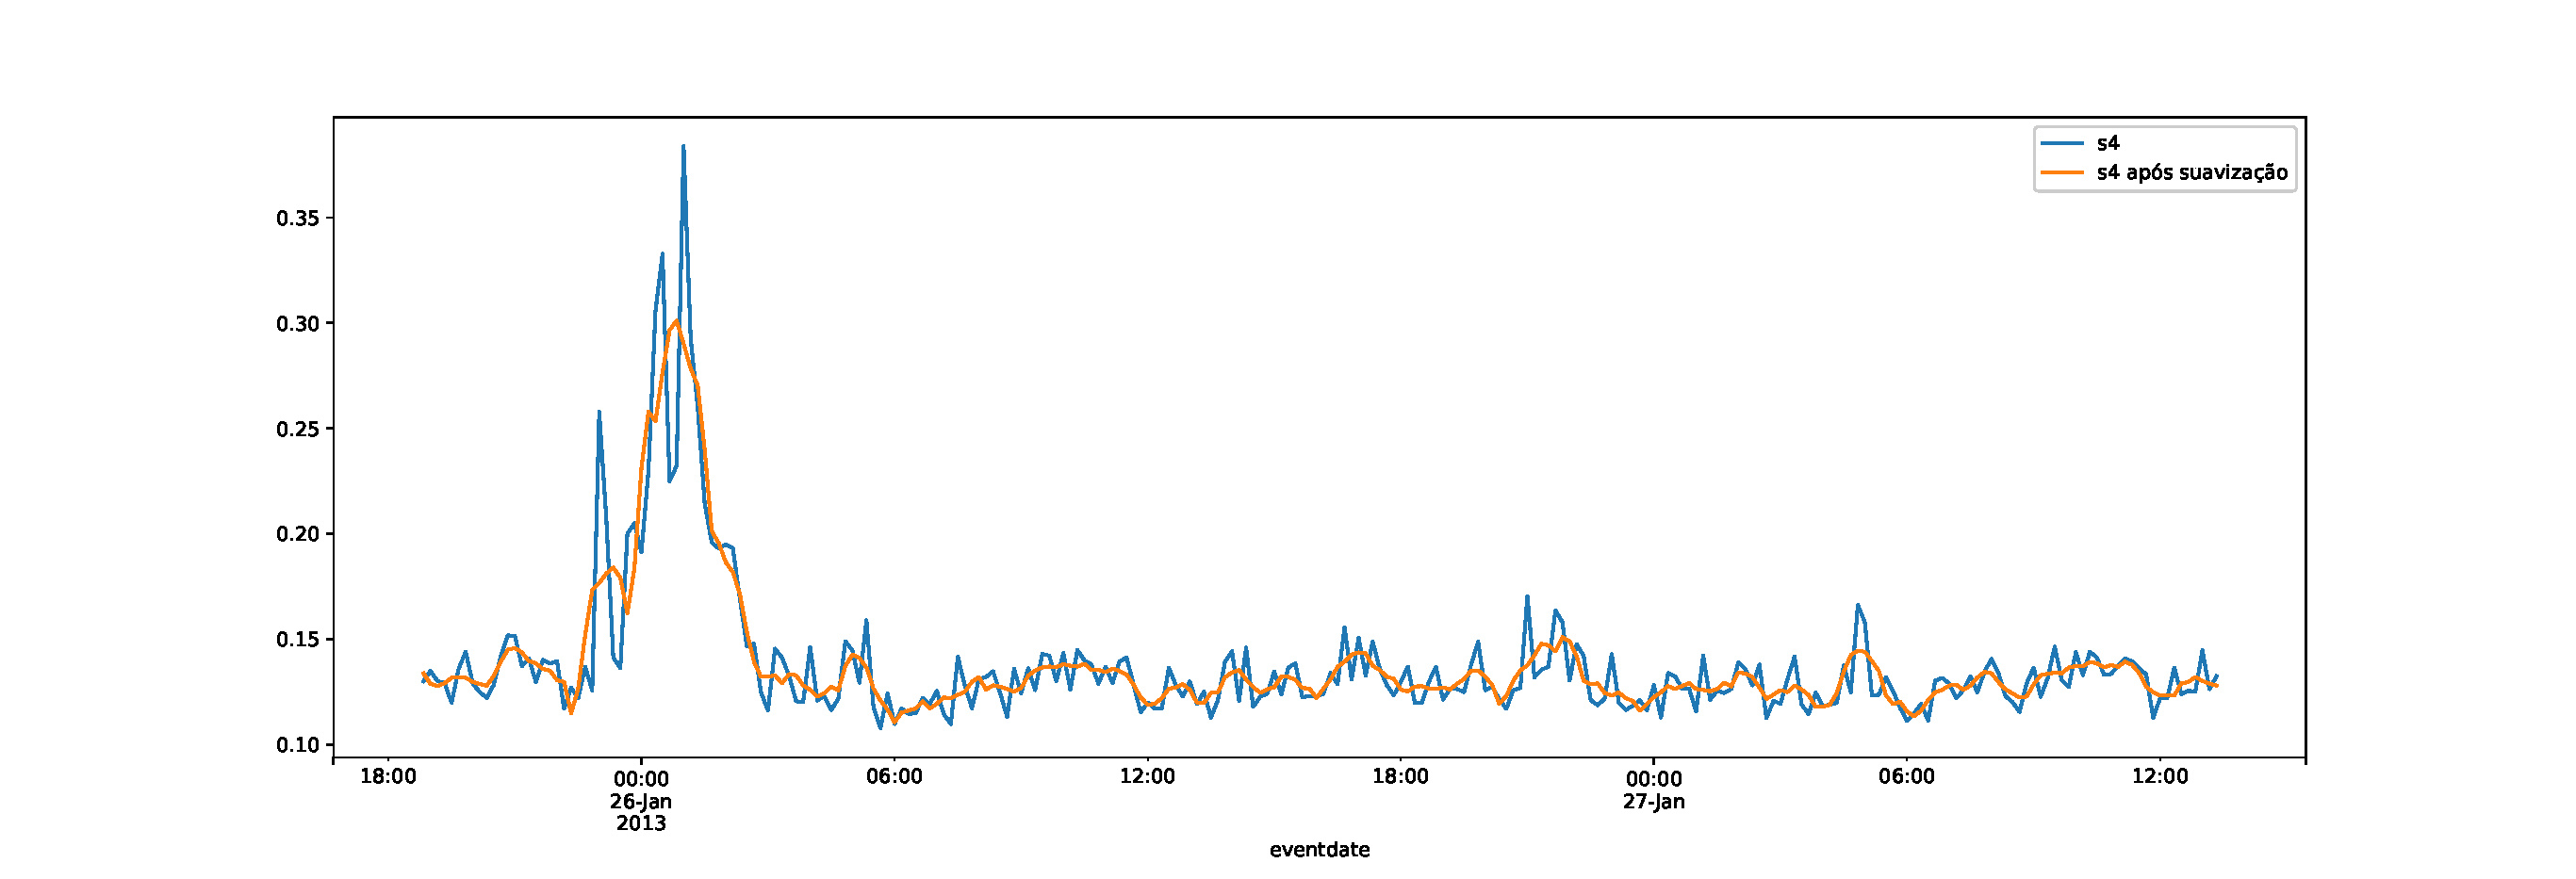
\includegraphics[width=1.4\linewidth]{./Figuras/s4_signal_noise_and_smooth_savgol.eps}}
\caption{A subfigure}
\label{fig:savgol}
\makebox[\textwidth][c]{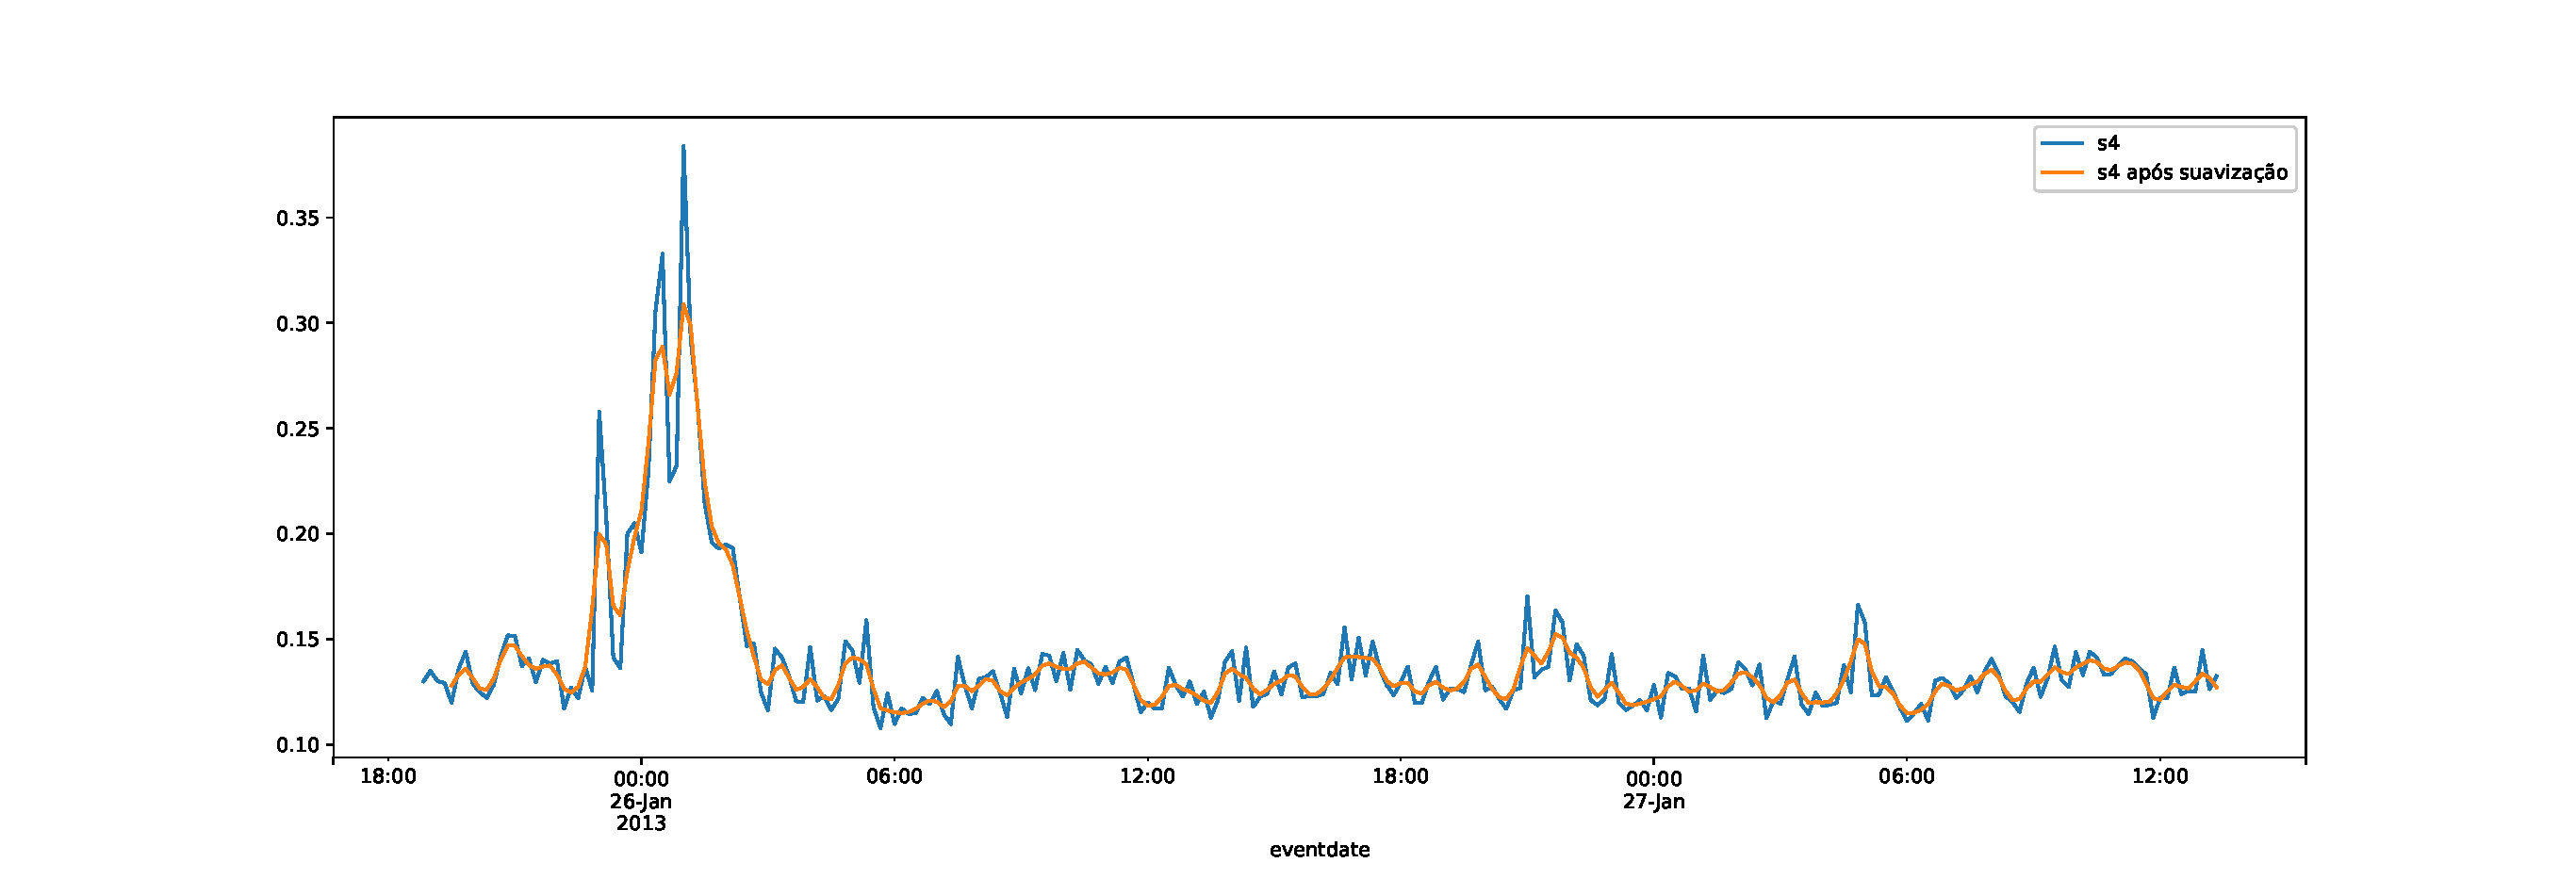
\includegraphics[width=1.4\linewidth]{./Figuras/s4_signal_noise_and_smooth_gaussian.eps}}
\caption{A subfigure}
\label{fig:gaussian}
\end{figure}

Finalmente, optou-se por utilizar uma combinação das duas técnicas de suavização aplicando primeiro do filtro de Savitzky–Golay seguido da média móvel com pesos gaussianos, ambos com os parâmetros especificados no parágrafo anterior.

Este notebook gera também uma tabela com todos os dados de S4, em passos de 10 min, onde as colunas representam o conjunto inicial de estações.

\section{Extração da série temporal de VTEC, para algumas estações}

O papel do notebook 03\_extract\_vtec\_stations.ipynb é o de extrair da série espaço-temporal do VTEC, séries temporais para as estações onde o índice S4 é medido. Estes dados então são preprocessados aplicando o mesmo processo de suavização utilizados nos dados de S4. Na figura \ref{fig:vtecsj2} é possível visualizar uma amostra do VTEC para São José dos Campos, juntamente com a aplicação separa das duas técnicas de suavização. Na figura \ref{fig:vtecsignal} há uma amostra do VTEC para o conjunto inicial de estações, observe que no intervalo entre às 9:00 e 15:00 UT o VTEC é aproximadamente igual entre as diversas estações, e que a partir das 18:00 UT os valores começam a divergir entre si, apresentado grandes diferenças após 00:00 até 06:00 UT, onde então começa a se agrupar novamente.

\begin{figure}[H]
\centering
\makebox[\textwidth][c]{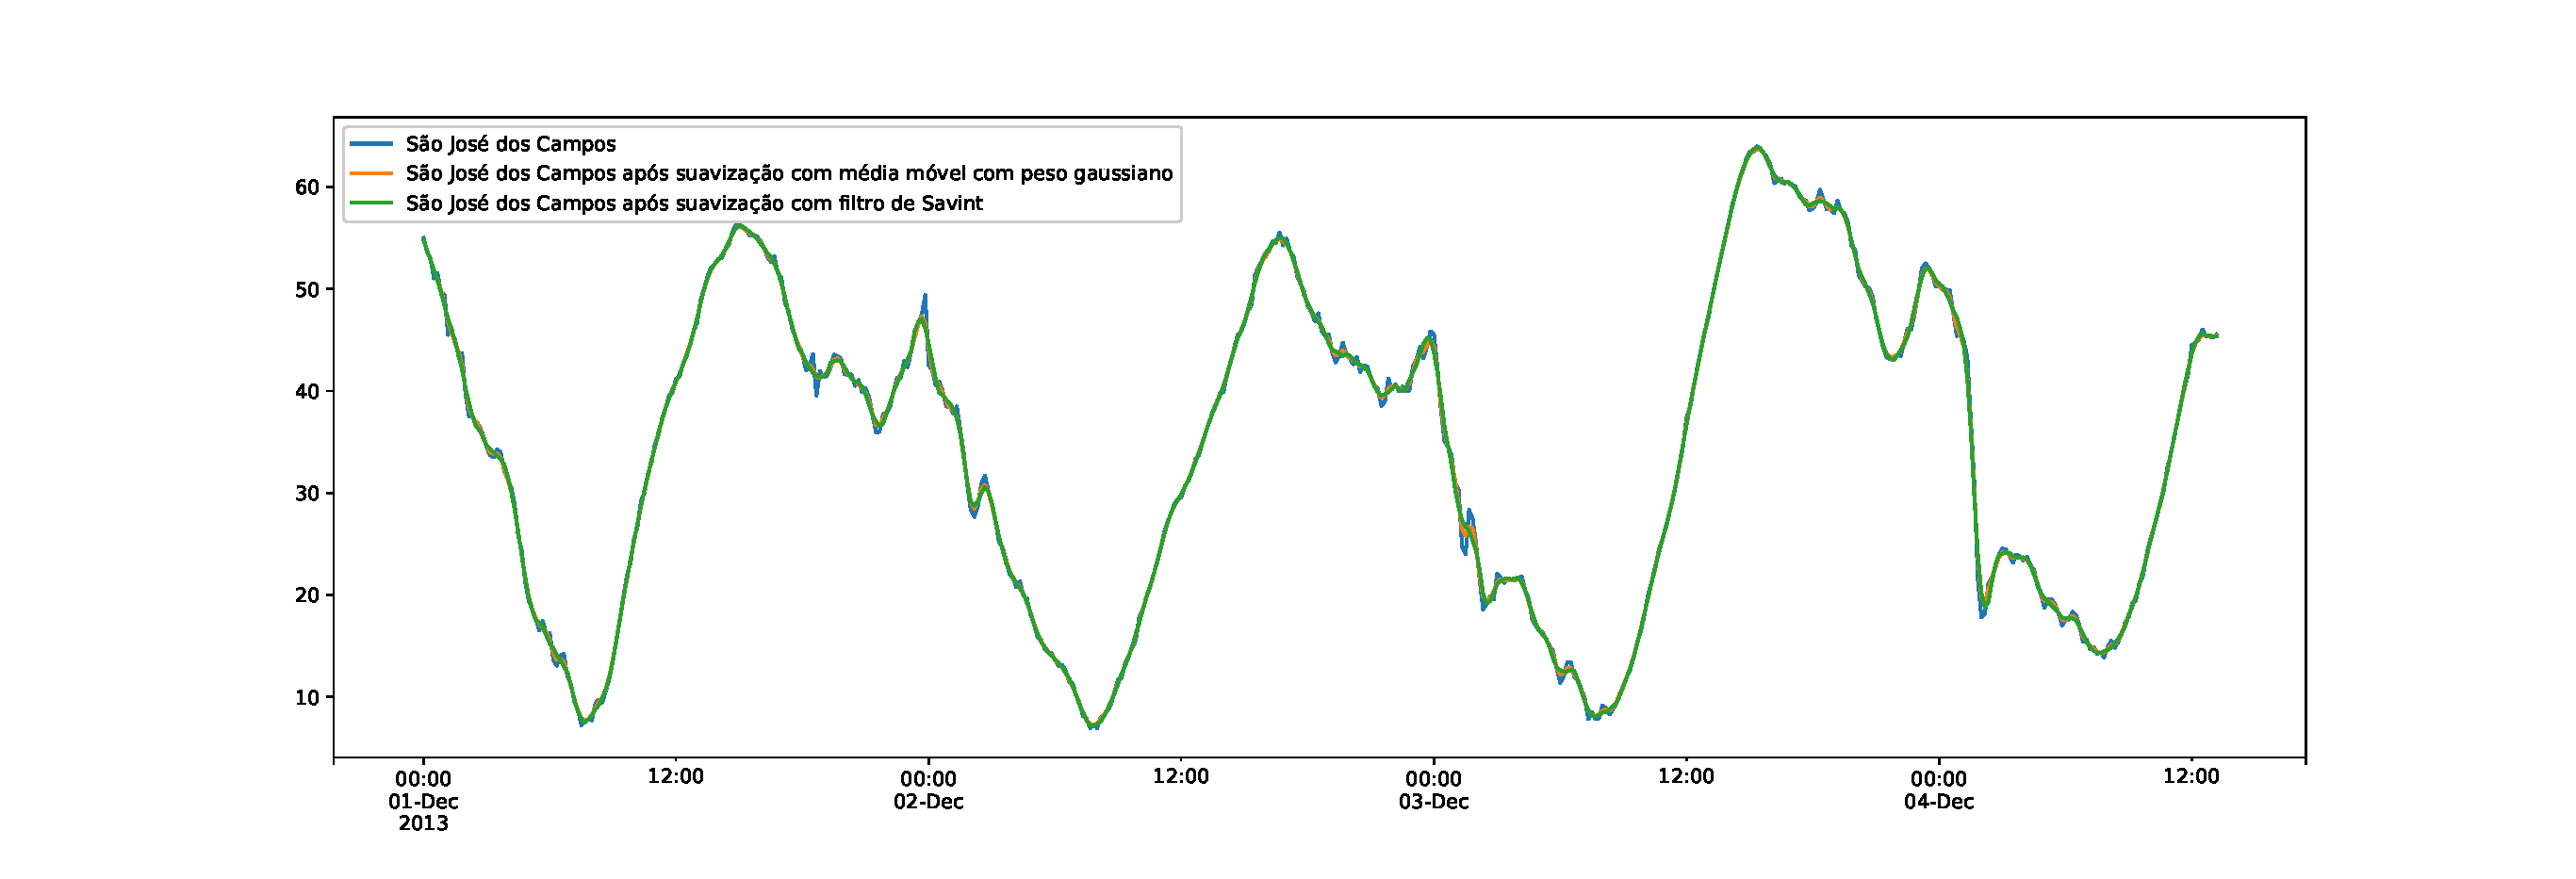
\includegraphics[width=1.5\columnwidth]{./Figuras/vtec_sj2.eps}}
\caption{A subfigure}
\label{fig:vtecsj2}
\makebox[\textwidth][c]{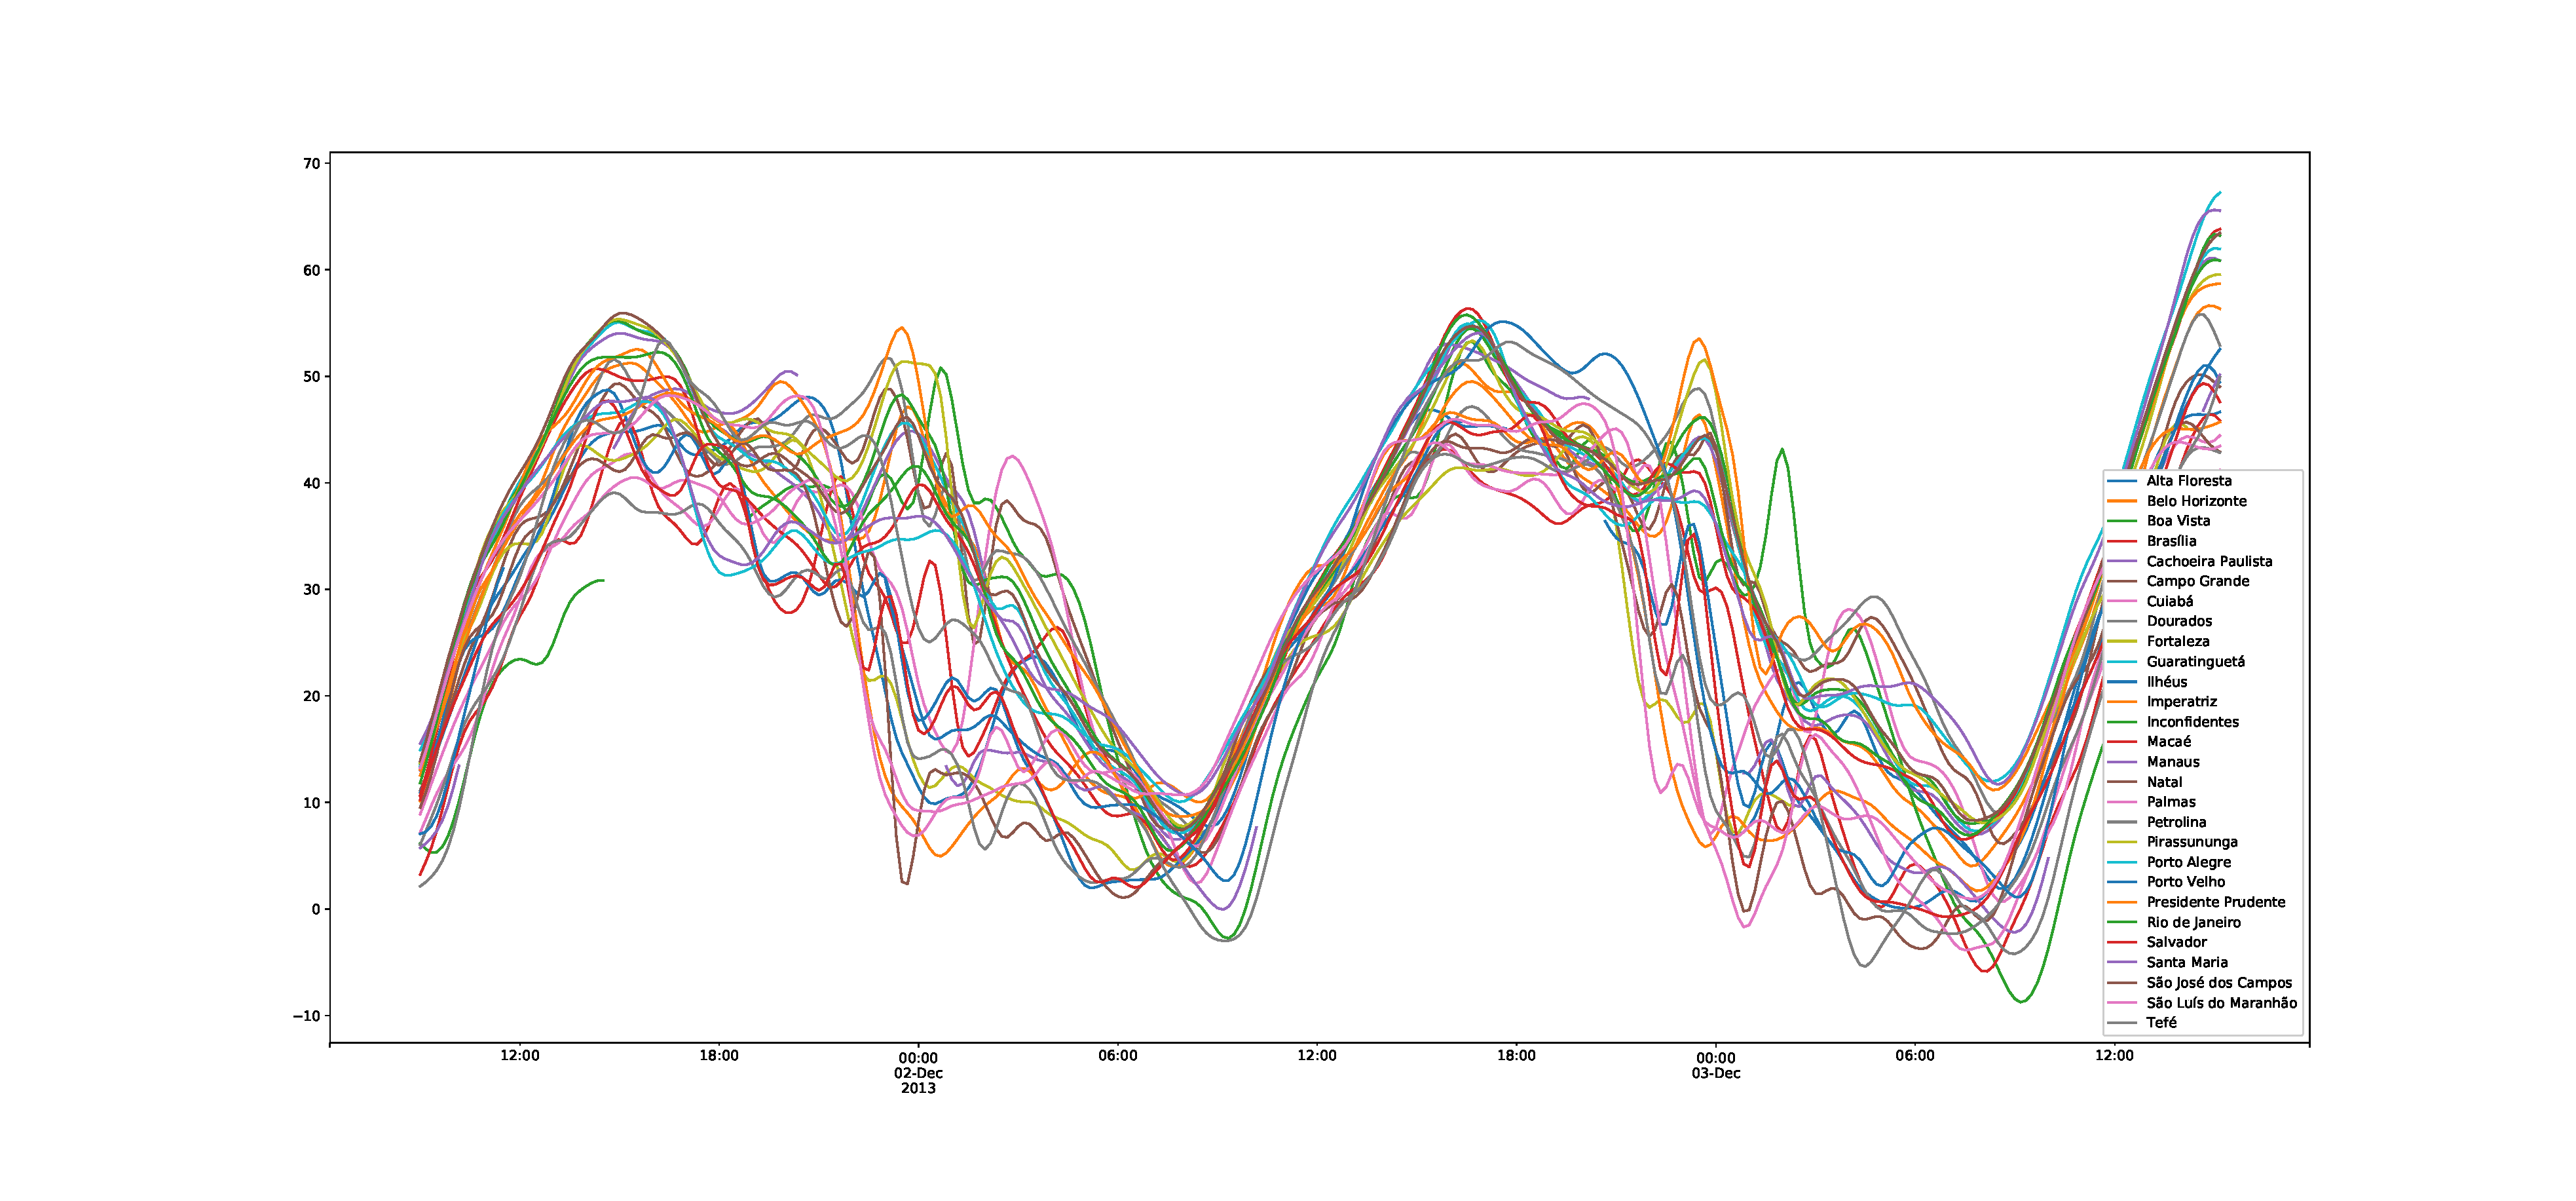
\includegraphics[width=1.5\columnwidth]{./Figuras/vtec_signal.eps}}
\caption{A subfigure}
\label{fig:vtecsignal}
\end{figure}

Em sua fase final este notebook gera uma tabela, onde cada coluna representa uma estação diferente com os dados de VTEC indexados pelo tempo, de modo que, pode-se falar em séries temporais para os dados de VTEC.

\section{Seleção fina dos dados de S4}

Após o pré-processamento dos dados de S4 é realizada uma seleção mais fina das estações que serão utilizadas neste trabalho, para tal foi empregado o notebook 04\_reanalize\_data.ipynb. O primeiro conjunto de estações descartas o foi, pois apresentava poucos pontos ao longo do período de janeiro de 2013 à dezembro de 2014 que levaram a curvas interpoladas que não são condizentes com a variável observada, o que foi evidenciado pela plotagem das séries temporais. O dados foram amostrados em um período menor, assim, foi realizado um recorte na série temporal de S4, de maneira a ambos terem o mesmo período de amostragem. Assim, o segundo conjunto de estações descartadas são as que não medidas no período de tempo selecionado. A tabela \ref{tab:stations} apresenta o grupo final de estações selecionados para o trabalho. As figuras \ref{fig:s4stations0}, \ref{fig:s4stations1} e \ref{fig:s4stations2} exibem a série temporal S4 para este grupo de estações, enquanto a figura \ref{fig:mapstationsre} apresenta um mapa com estas.

\begin{table}
\addtolength{\leftskip} {-2cm} % increase (absolute) value if needed
\addtolength{\rightskip}{-2cm}
\small
\begin{tabular}{|l|l|l|c|c|c|c|c|}
\hline
Cidade              & Est.  & Cód. de Id.           &  Alt.     &   Lat.     &  Lon.      &  Lat. Mag.    &  Lon. Mag.       \\ \hline
Belo Horizonte      &    MG &                   bhz &   858.000 & -19.868500 & -43.954200 &    -25.426147 &      24.786619   \\ \hline
Brasília            &    DF &                   bsa &  1050.000 & -15.764200 & -47.869400 &    -24.348659 &      22.352744   \\ \hline
Cachoeira Paulista  &    SP &                   cpa &   580.000 & -22.410000 & -45.000000 &    -24.456556 &      22.960540   \\ \hline
Campo Grande        &    MS &                    32 &       NaN & -20.497000 & -54.615000 &    -21.417704 &      14.873907   \\ \hline
Cuiabá              &    MT &                   cub &   278.000 & -15.555200 & -56.069800 &    -14.336068 &      14.530440   \\ \hline
Dourados            &    MS &                   dou &   756.120 & -22.110000 & -54.550000 &    -23.627266 &      14.698554   \\ \hline
Fortaleza           &    CE &                    24 &       NaN &  -3.742000 & -38.539000 &           NaN &            NaN   \\ \hline
Guaratinguetá       &    SP &                    33 &       NaN & -22.789000 & -45.220000 &    -24.188879 &      22.620120   \\ \hline
Ilhéus              &    BA &                   ios &     0.000 & -14.470000 & -39.100000 &    -13.470248 &      30.548727   \\ \hline
Inconfidentes       &    MG &                    25 &       NaN & -22.318000 & -46.329000 &    -26.299459 &      22.004117   \\ \hline
Macaé               &    RJ &                    11 &       NaN & -22.823000 & -41.785700 &    -20.542047 &      25.191448   \\ \hline
Natal               &    RN &                   nta &     0.000 &  -5.836162 & -35.121000 &           NaN &            NaN   \\ \hline
Palmas              &    RO &                     3 &       NaN & -10.200000 & -48.312000 &    -12.264838 &      23.425112   \\ \hline
Pirassununga        &    SP &                    30 &       NaN & -21.989000 & -47.334000 &    -23.990783 &      21.003125   \\ \hline
Porto Alegre        &    RS &                     4 &       NaN & -30.071000 & -51.119000 &    -22.954879 &      15.550843   \\ \hline
Presidente Prudente &    SP &                     6 &       NaN & -22.120000 & -51.407000 &    -21.640946 &      17.249042   \\ \hline
Rio de Janeiro      &    RJ &                    34 &       NaN & -22.823000 & -43.238000 &    -20.105803 &      23.888647   \\ \hline
Salvador            &    BA &                    26 &       NaN & -13.001000 & -38.508000 &    -12.123350 &      31.680944   \\ \hline
Santa Maria         &    RS &                   sta &   110.100 & -29.712591 & -53.717206 &    -22.659740 &      13.628064   \\ \hline
São José dos Campos &    SP &                   sj2 &   593.440 & -23.207000 & -45.859000 &    -24.835610 &      22.002028   \\ \hline
Tefé                &    AM &                   tfe &     0.057 &  -3.180000 & -64.440000 &      6.385157 &       9.314963   \\ \hline
\end{tabular}\label{tab:stations}
\begin{tabular}{|l|c|c|c|}
\hline
Cidade              &   Alt. da Cidade &  Lat. da Cidade &  Lon. da Cidade \\ \hline
Belo Horizonte      &            767.0 &       -19.81570 &        -43.9542 \\ \hline
Brasília            &           1130.0 &       -15.78010 &        -47.9292 \\ \hline
Cachoeira Paulista  &            545.0 &       -22.67370 &        -44.9973 \\ \hline
Campo Grande        &            612.0 &       -20.44350 &        -54.6478 \\ \hline
Cuiabá              &            180.0 &       -15.59890 &        -56.0949 \\ \hline
Dourados            &            448.0 &       -22.22180 &        -54.8064 \\ \hline
Fortaleza           &             14.0 &        -3.71839 &        -38.5434 \\ \hline
Guaratinguetá       &            526.0 &       -22.81620 &        -45.1935 \\ \hline
Ilhéus              &              9.0 &       -14.79730 &        -39.0355 \\ \hline
Inconfidentes       &            864.0 &       -22.31710 &        -46.3284 \\ \hline
Macaé               &              7.0 &       -22.37170 &        -41.7857 \\ \hline
Natal               &             38.0 &        -5.79448 &        -35.2110 \\ \hline
Palmas              &            260.0 &       -10.16890 &        -48.3317 \\ \hline
Pirassununga        &            625.0 &       -21.99600 &        -47.4268 \\ \hline
Porto Alegre        &             22.0 &       -30.02770 &        -51.2287 \\ \hline
Presidente Prudente &            471.0 &       -22.12760 &        -51.3856 \\ \hline
Rio de Janeiro      &             20.0 &       -22.90350 &        -43.2096 \\ \hline
Salvador            &             12.0 &       -12.97040 &        -38.5124 \\ \hline
Santa Maria         &            139.0 &       -29.69140 &        -53.8008 \\ \hline
São José dos Campos &            593.0 &       -23.17910 &        -45.8872 \\ \hline
Tefé                &             28.0 &        -3.32073 &        -64.7236 \\ \hline
\end{tabular}
\label{tab:stations}
\end{table}

\begin{figure}[H]
\centering
\makebox[\textwidth][c]{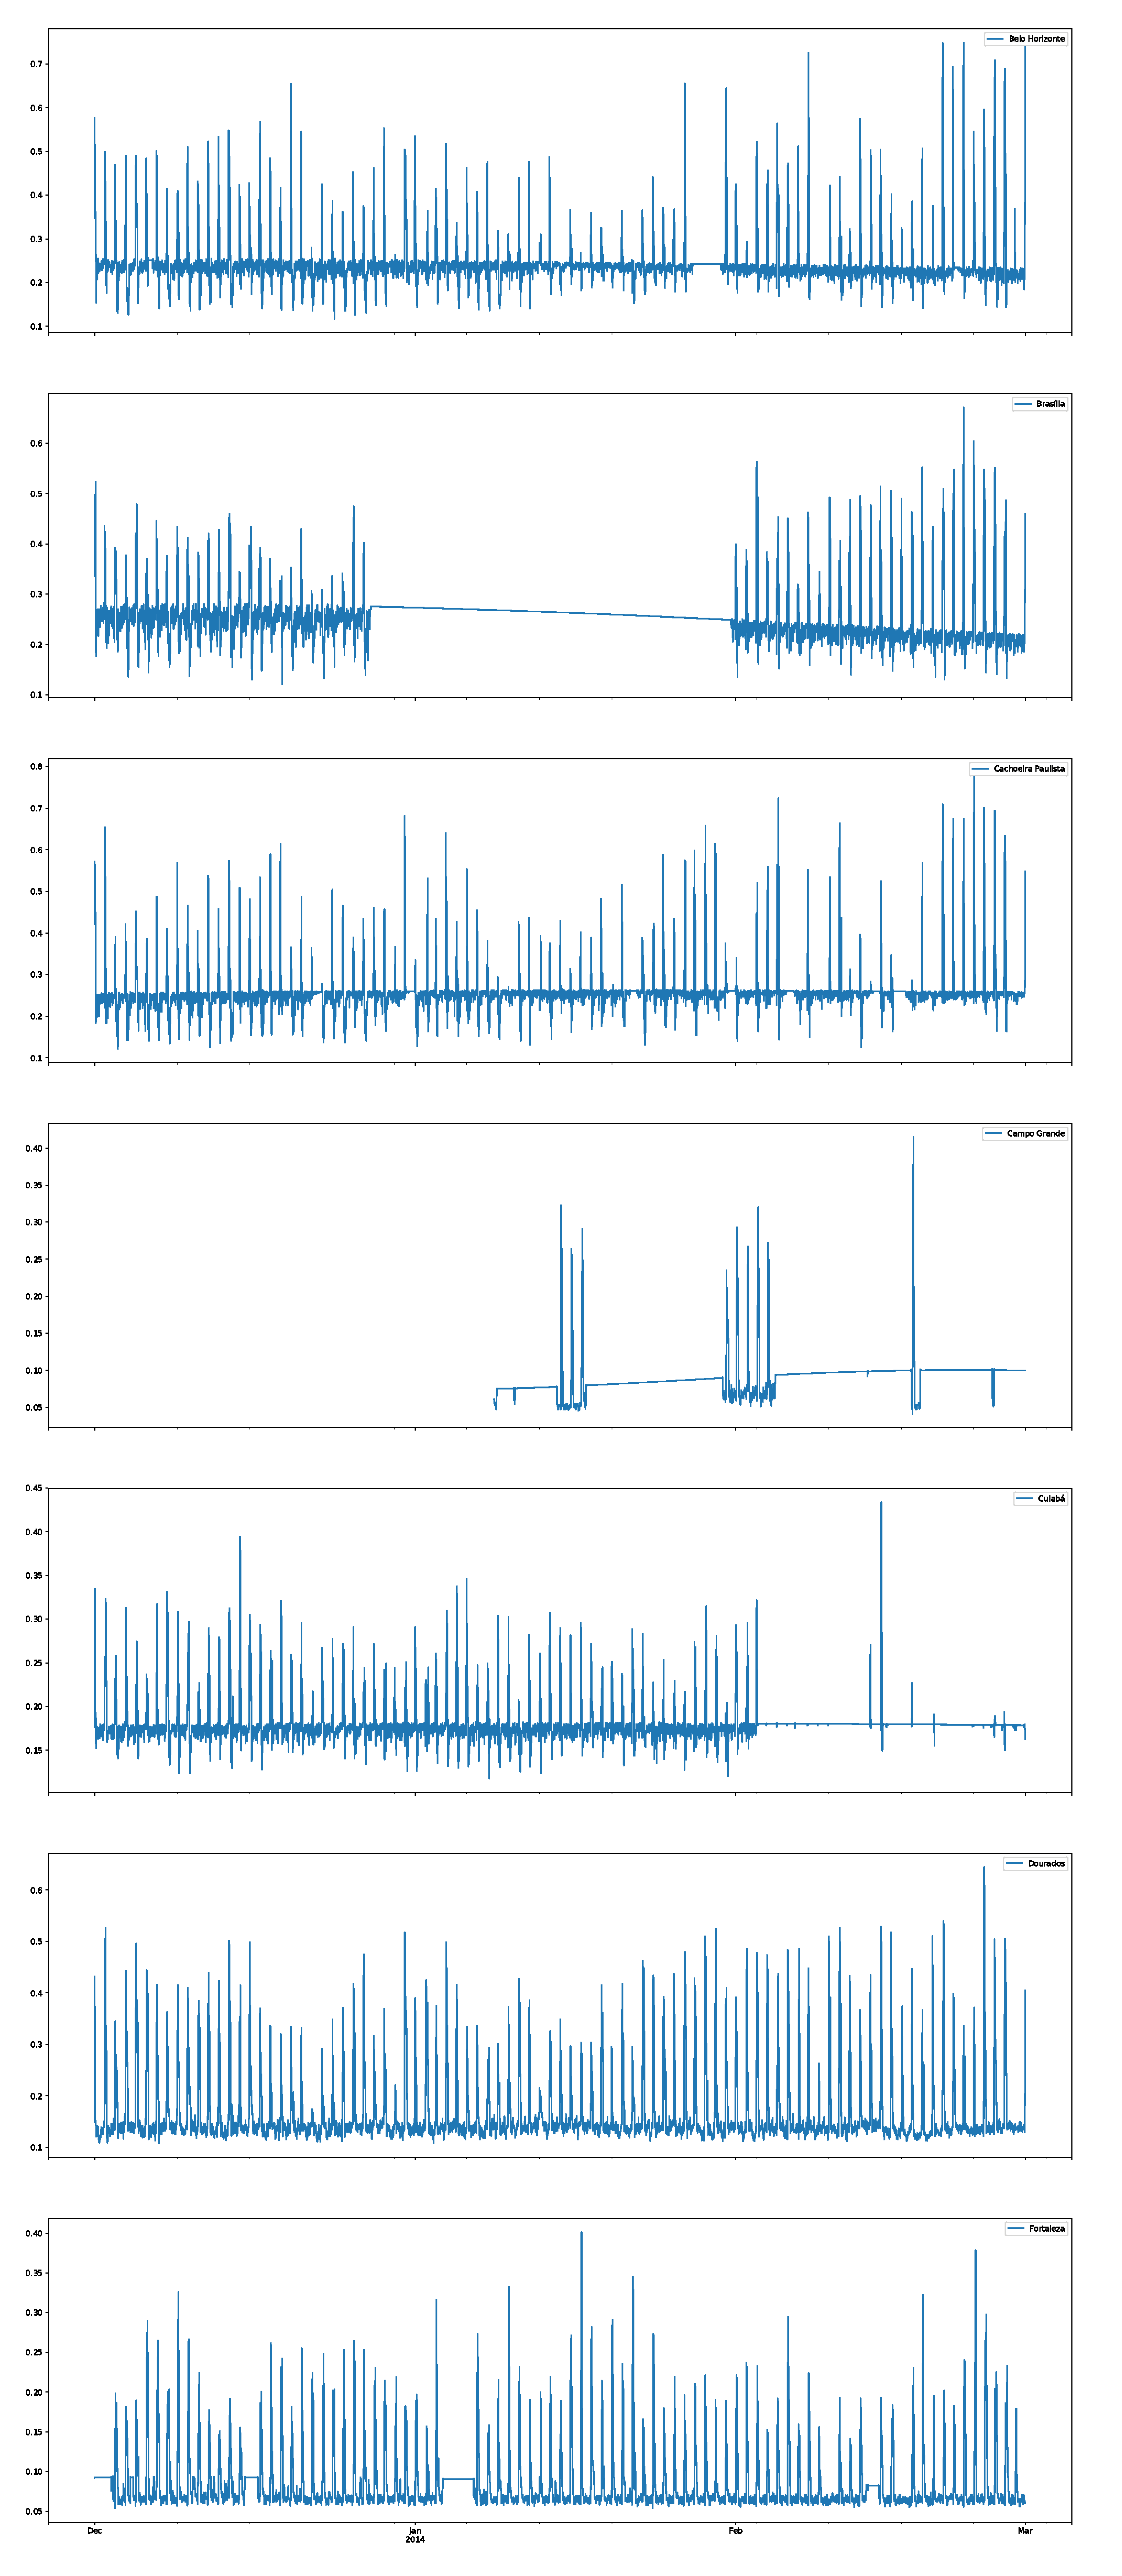
\includegraphics[width=1.0\columnwidth]{./Figuras/s4_stations0.eps}}
\label{fig:s4stations0}
\caption{A subfigure}
\end{figure}

\begin{figure}[H]
\centering
\makebox[\textwidth][c]{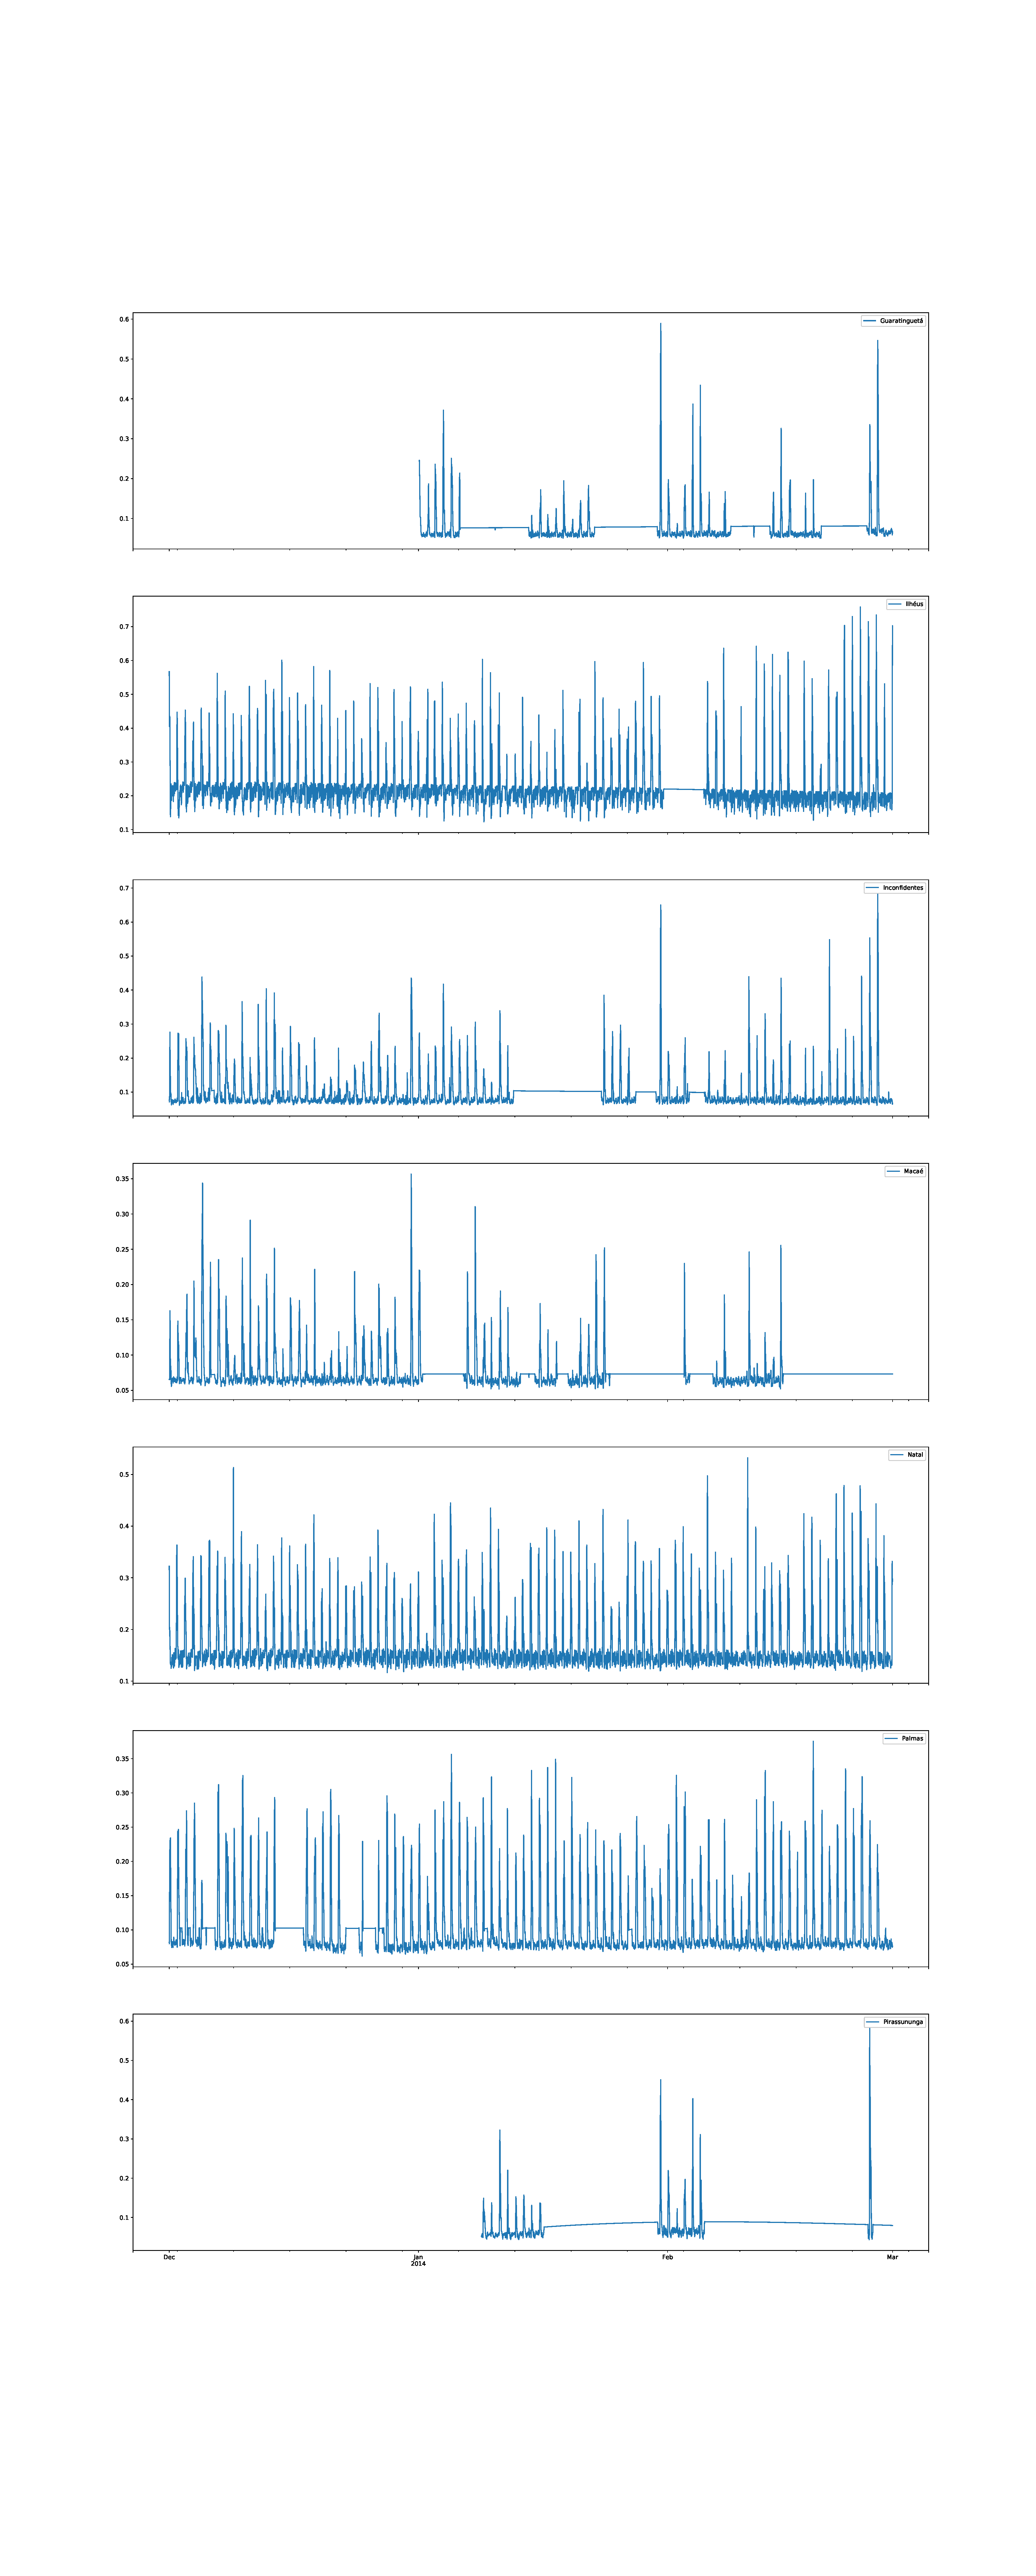
\includegraphics[width=1.5\columnwidth]{./Figuras/s4_stations1.eps}}
\label{fig:s4stations1}
\caption{A subfigure}
\end{figure}

\begin{figure}[H]
\centering
\makebox[\textwidth][c]{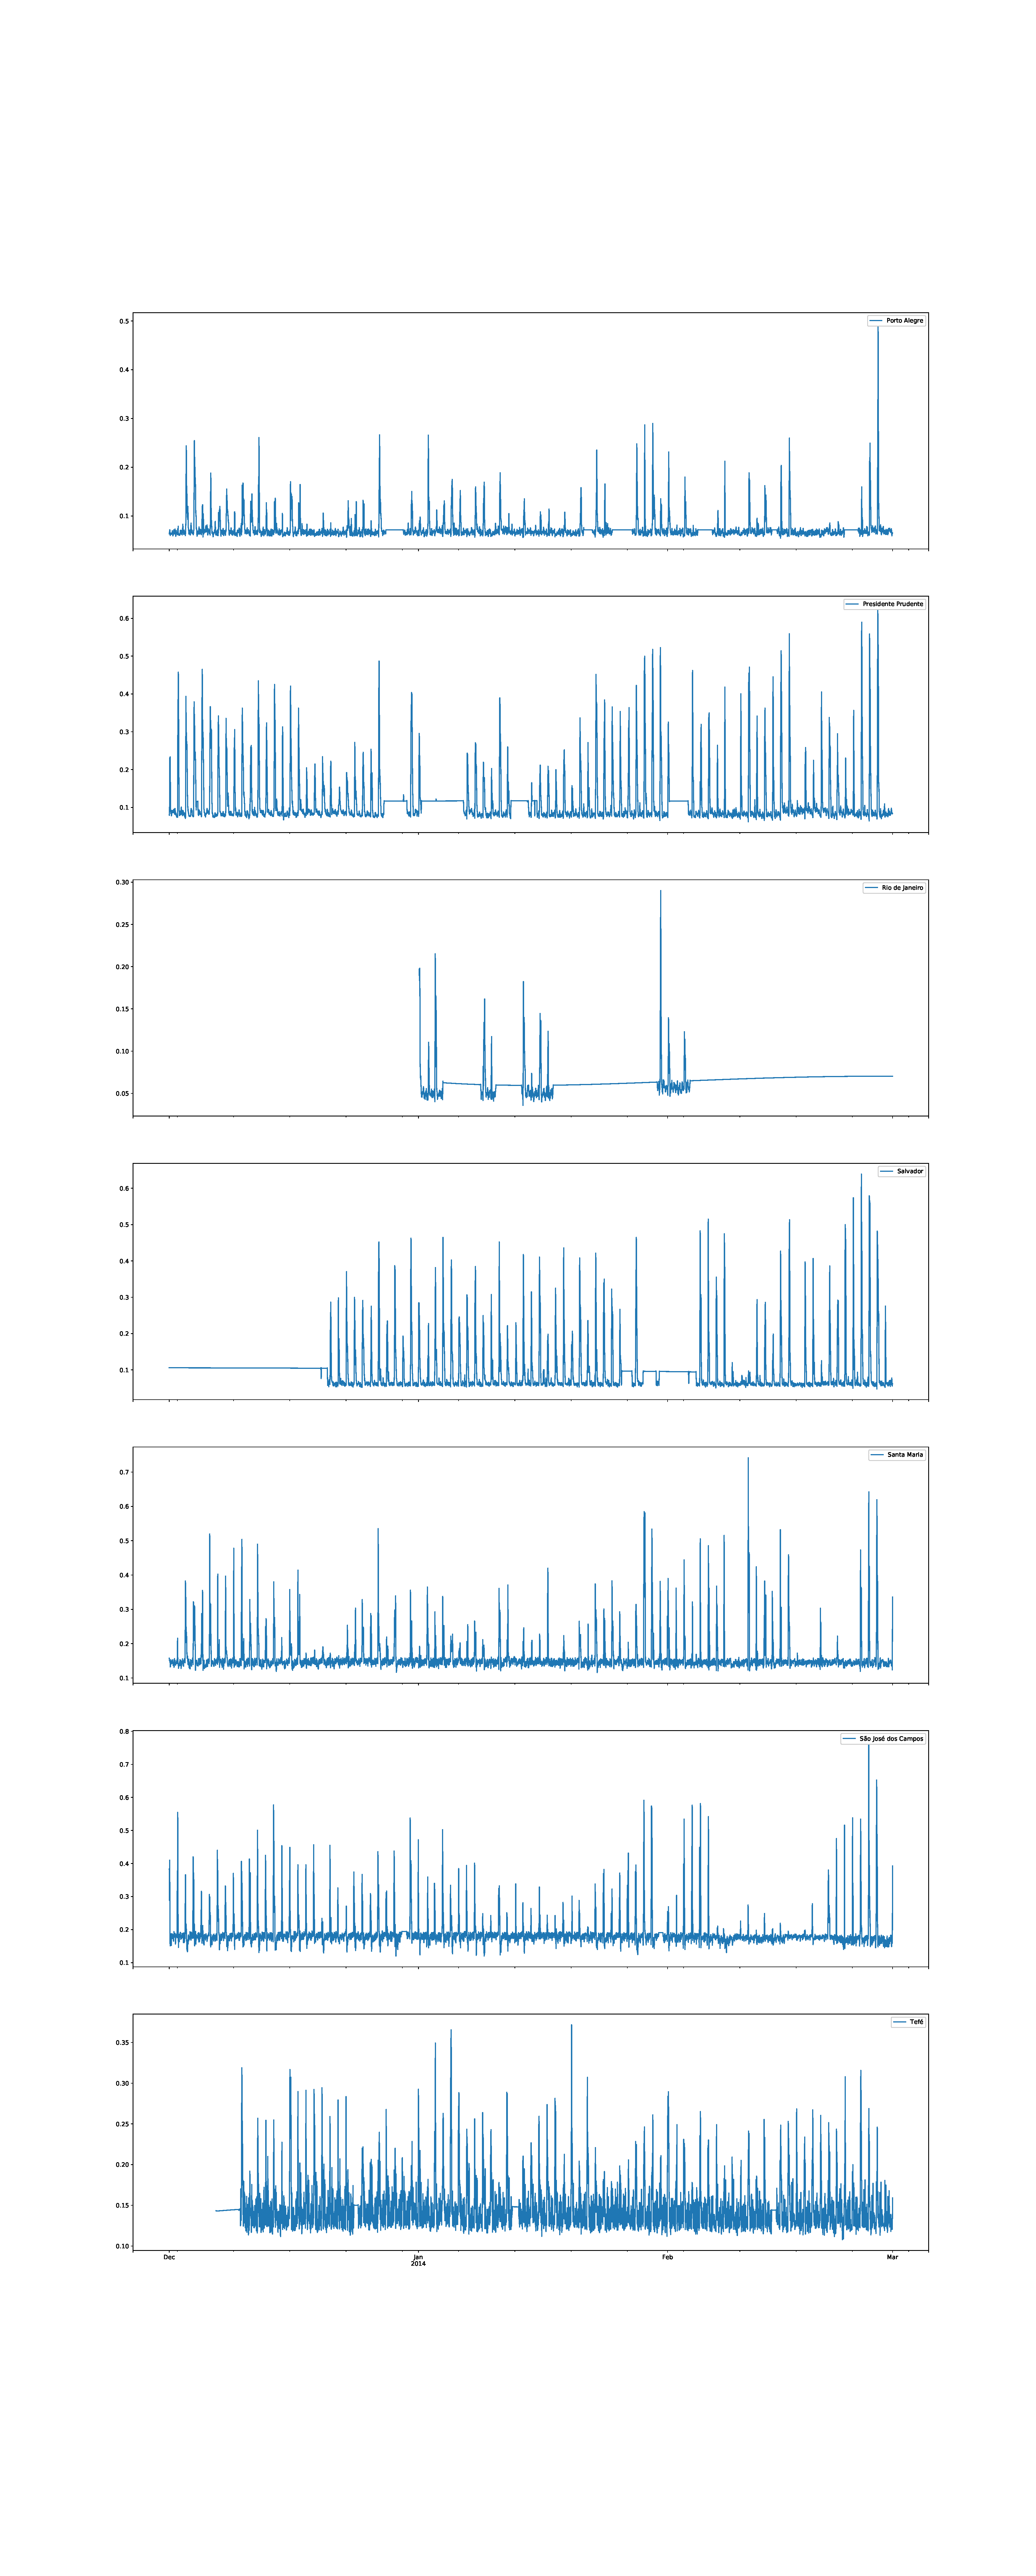
\includegraphics[width=1.5\columnwidth]{./Figuras/s4_stations2.eps}}
\label{fig:s4stations2}
\caption{A subfigure}
\end{figure}

\begin{figure}[h]
\centering
\makebox[\textwidth][c]{\includesvg[width=1.6\columnwidth]{./Figuras/map_stations_re.svg}}
\label{fig:mapstationsre}
\caption{A subfigure}
\end{figure}

\section{Visualizando S4  e VTEC}\label{sec:viss4vtec}

Feita uma seleção mais fina das estações que fornecerão as séries temporais de S4, assim, como um recorte adequado no tempo, é adequado plotar a série temporal do VTEC, juntamente com a do S4. Esta etapa é realizada no notebook 05\_visualize\_vtec\_s4\_data. Os gráficos são feitos em dois grupos distintos, o primeiro apresenta uma amostra das séries temporais, fornecendo um resolução visual melhor, enquanto o segundo fornece a série completa. Algumas observações pode ser feitas analisando visualmente ambos os conjuntos. Nota-se, por exemplo:

\begin{itemize}
\item uma periodicidade em ambos os dados; 
\item os valores de S4 sobem conforme o do VTEC diminui;
\item os valores de pico de S4 aparecem em quedas e mínimos do VTEC;
\item os dados de S4 apresentam maior ruído e menor disponibilidade;
\item flutuações mais intensas do S4 aparecem no máximo do VTEC.
\end{itemize}

\section{Análises: S4$\times$VTEC em São José dos Campos}

Existem várias formas de se buscar por padrões e correlações em um conjunto de dados, tal como a visualização por meio da plotagem de um gráfico representativo de uma série temporal. Assim, a seção \ref{sec:viss4vtec} forneceu um indicativo da correlação em sua conclusão. Observado tal fato o próximo passo é buscar por um modelo que faça um mapeamento entre VTEC e S4. Este pode ter como conjunto de entrada o valor de VTEC e o de saída o S4, uma vez que ambas as variáveis são contínuas se busca realizar uma regressão. 

Poder-se-ia buscar um mapeamento tal que a cada valor de VTEC seja associado um valor de S4 por estação, entretanto, usando os padrões observados juntamente das referências \cite{}, derivou-se um conjunto adicional de variáveis, que são a derivada temporal primeira e segunda do VTEC, a diferença do VTEC entre São José dos Campos e Pirassununga, a diferença do VTEC entre São José dos Campos e Brasília, assim como as derivadas temporais primeira de ambas as diferenças. 

As derivadas temporais são interessantes, pois os valores de S4 aumentam conforme o valor de VTEC diminui, portanto existe uma variação no tempo que pode ser melhor extraída pela derivada temporal. As bolhas ionosféricas se deformam e propagam ao longo de um meridiano magnético, as estações de Brasília, Pirassununga e São José dos Campos se encontram aproximadamente sobre o mesmo meridiano magnético, usando ambos os fatos considere que exista uma bolha em Brasília, e não em São José dos Campos, a diferença de VTEC terá um valor positivo, enquanto que se estiverem em ambas as cidades se tem um valor aproximadamente nulo, e com a bolha apenas em São José dos Campos um valor de diferença negativa, isto exibe claramente a propriedade da diferença espacial do VTEC em mapear a localização da bolha. A derivada temporal das diferenças espaciais fornece um indicativo da dinâmica da bolha.

Sumarizando, ficou-se com o seguinte conjunto de variáveis/atributos, mais uma variável alvo S4:

\begin{itemize}
\item {\bf vtec} - conteúdo eletrônico total vertical;
\item {\bf vtec\_dt} - diferença finita de primeira ordem no tempo do VTEC, calculada por $vtec_i-vtec_{i-1}$;
\item {\bf vtec\_dt2} - diferença finita de segunda ordem no tempo do VTEC, calculada por $vtec_{i+1}-2vtec_i+vtec_{i-1}$;
\item {\bf gvtec1} - diferença entre o VTEC de São José dos Campos e Pirassununga;
\item {\bf gvtec1\_dt} - diferença finita de primeira ordem no tempo do gvtec1, calculada por $gvtec1_i-gvtec1_{i-1}$;
\item {\bf gvtec2} - diferença entre o VTEC de São José dos Campos e Brasília;
\item {\bf gvtec2\_dt} - diferença finita de primeira ordem no tempo do gvtec1, calculada por $gvtec2_i-gvtec2_{i-1}$;
\item {\bf S4} - índice de cintilação ionosférico em São José dos Campos;
\end{itemize}

O papel do notebook 06\_analise\_sj2.ipynb é o de construir as variáveis definidas acima, assim como o de concatenar tais variáveis em uma tabela que possa ser utilizada em algoritmos de aprendizagem de maquina para desenvolvimento de um modelo.

Em posse desse conjunto de variáveis utilizou-se de um método de normalização para restringir o valor destas ao intervalo $[0,1]$ seguindo do treinamento de uma árvore de regressão, uma floresta randômica de regressão e uma máquina de suporte vetorial também de regressão. Esses modelos foram desenvolvidos respectivamente nos notebooks 07\_analise\_sj2\_tree.ipynb, 07\_analise\_sj2\_random\_forest.ipynb e 07\_analise\_sj2\_svm.ipynb. Além disso, para todos os modelos seguiu-se com uma análise de sensibilidade aos atributos, removendo uma de cada vez e reavaliando as métricas do modelo gerado.



%% insira quantos capítulos desejar com o seguinte comando:
%\include{_pasta_do_arquivo_/_meu_arquivo_} %%sem a extensão
%% note que deverá haver um arquivo _meu_arquivo_.tex (com extensão) no diretório _pasta_do_arquivo_

%\include{./docs/conclusao}

%% Bibliografia %% não alterar %% obrigatório %testebib
\bibliography{./bib/referencia} %% aponte para seu arquivo de bibliografia no formato bibtex (p.ex: referencia.bib)


%\include{./docs/glossario} %% insira os termos do glossário no arquivo glossario.tex %% opcional

\inicioApendice %% opcional, comente esta linha e a seguintes se não houver apendice(s)
%%%%%%%%%%%%%%%%%%%%%%%%%%%%%%%%%%%%%%%%%%%%%%%%%%%%%%%
%Apêndice A
\hypertarget{estilo:apendice1}{} %% uso para este Guia
%Este apêndice foi criado apenas para indicar como construir um apêndice no estilo, não existia no original da tese.
%%%%%%%%%%%%%%%%%%%%%%%%%%%%%%%%%%%%%%%%%%%%%%%%%%%%%%
\renewcommand{\thechapter}{}%
\chapter{APÊNDICE A - AUTORIZAÇÃO PARA PUBLICAÇÃO}	% trocar A por B na próxima apêndice e etc
\label{apendiceA}	% trocar A por B na próxima apêndice e etc
\renewcommand{\thechapter}{A}%		% trocar A por B na próxima apêndice e etc

Há dois formulários de autorização para publicação, um para publicações de trabalhos acadêmicos e outro para publicações técnico-científicas, neste apêndice encontram-se os modelos dos formulários e suas respectivas instruções de preenchimento. 

\section{Autorização para Publicação de Trabalho Acadêmico - INPE-393}

\label{instr393}

	\begin{figure}[ht]
		\caption{Formulário Autorização para Publicação de Trabalho Acadêmico INPE-393.}
		\vspace{6mm}	% acrescentar o espaçamento vertical apropriado entre o título e a borda superior da figura
		\centering
   		\includegraphics[height=16cm]{./Figuras/form393.png}	   
 		\label{form393}
	\end{figure}


\subsection{Instruções do Formulário INPE-393} 

\begin{enumerate} 

 \item \textbf{série:} com este número o SID identifica as publicações do INPE, composto da sigla da Instituição, número sequencial geral da publicação, sigla e número sequencial do tipo de publicação, exemplo: INPE-14209-TDI/1110;
 
 \item \textbf{número:} será composto da sigla da unidade do SID, mais 4 (quatro) dígitos e do ano em curso. Este número de referência é de controle da unidade emissora. Ex.: SID-0001/2007;

 \item \textbf{título da publicação:} deve ser completo, evitando-se abreviar palavras;

 \item \textbf{nome do autor e do orientador:} estes campos devem ser preenchidos por extenso, da mesma forma em que irão constar da publicação;

 \item \textbf{origem da publicação:} sigla da unidade do servidor (autor da publicação), conforme TQ-001;

 \item \textbf{curso:} sigla do curso, de acordo com a Estrutura de Divisão de Trabalho - EDT do INPE;
 
 \item \textbf{tipo:} assinalar se é tese ou dissertação;

 \item \textbf{apresentação:} colocar a data de aprovação final;

 \item \textbf{revisão técnica:} o responsável designado pela Banca Examinadora para verificação de correções e, na ausência desse, o orientador da tese ou dissertação deve
carimbar, datar e assinar após a versão \emph{on line} do trabalho;

 \item \textbf{revisão de linguagem:} o responsável designado pela Banca Examinadora para verificação de correções, e na ausência deste o orientador deve assinalar a solicitação ou a dispensa da revisão de linguagem e, carimbar, datar e assinar; o revisor deve datar e assinar após a revisão;
 
 \item \textbf{distribuição:} O SID deve informar a quantidade de CD's e de cópias impressas da tese ou dissertação, conforme lista de distribuição;
 
 \item \textbf{verificação de normalização:}  Após a verificação da versão \emph{on line} do trabalho quanto às normas editoriais, o SID deve datar e assinar;
 
 \item \textbf{autorização final:} data e assinatura do Titular de Nível A, conforme TQ-001, a que o Serviço de Pós-Graduação estiver subordinado.
 
 \item \textbf{observações:} para outras informações necessárias. 

\end{enumerate}

\section{Autorização para Publicação - INPE-106}
\begin{figure}[ht!]
	\caption{Formulário Autorização para Publicação de Trabalho Acadêmico INPE-106 folha 1.} 
	\vspace{6mm}	% acrescentar o espaçamento vertical apropriado entre o título e a borda superior da figura
	\centering
	\includegraphics[height=18cm]{./Figuras/form106.png}
	\label{form106}
\end{figure}

\begin{figure}[ht!]
	\caption{Formulário Autorização para Publicação de Trabalho Acadêmico INPE-106 folha 2.} 
	\vspace{6mm}	% acrescentar o espaçamento vertical apropriado entre o título e a borda superior da figura
	\centering
	\includegraphics[height=18cm]{./Figuras/form106folha2.png}
	\label{form106a}
\end{figure}

\clearpage
\subsection{Instruções do Formulário INPE-106} 
\label{instr106}


\begin{enumerate}

 \item \textbf{série:} com este número o SID identifica as publicações do INPE, composto da sigla da Instituição, número sequencial geral da publicação, sigla e número sequencial do tipo de publicação, exemplo: INPE-5616-RPQ/671. 
 
 \item \textbf{número:} será composto da sigla da unidade constante da Estrutura Organizacional do INPE (TQ-001), mais 4 (quatro) dígitos e do ano em curso. Este número de referência é de controle da unidade solicitante. Ex: CEA-0001/2007;
 
 \item \textbf{título da publicação:} deve ser completo, evitando-se abreviar palavras;

 \item \textbf{nome do autor, tradutor e editor:}  estes campos devem ser preenchidos por extenso, da mesma forma em que irão constar da publicação;

 \item \textbf{origem da publicação:} sigla da unidade do servidor (autor da publicação), conforme TQ-001;

 \item \textbf{projeto:} sigla do projeto de acordo com a Estrutura de Divisão de Trabalho - EDT do INPE;

 \item \textbf{tipo de publicação:} assinalar o tipo de publicação proposta:

 \begin{enumerate}
  \item{Relátorio de Pesquisa (RPQ)},
  \item{Notas Técnico-Científicas (NTC)},
  \item{Propostas e Relatórios de de Projeto (PRP)},
  \item{Manuais Técnicos (MAN)},
  \item{Publicações Didáticas (PUD)},
  \item{Trabalhos Acadêmicos Externos (TAE)}.
 \end{enumerate}

 \item \textbf{divulgação:} assinalar, de acordo com os critérios de classificação. Se houver Lista de Divulgação, nesta deverá constar os nomes e endereços completos;

 \item \textbf{convênio:} descrever o nome da instituição, quando a publicação for realizada pelo INPE e outra organização, preencher somente para o tipo PRP; 
 
    \item \textbf{autorização preliminar:} data, carimbo e assinatura do Titular da Unidade a que o autor esteja subordinado e, assinatura do revisor que efetuou a revisão técnica aprovando a versão \emph{on line} do trabalho e do revisor que realizou a revisão de linguagem, quando solicitadas; 
    
  \item \textbf{verificação de normalização:} o SID deve datar e assinar após a revisão da adequação às normas editoriais;   
  
  \item \textbf{distribuição:} O SID deve informar a quantidade de CD's e de cópias impressas que deverão ser gravados conforme lista de distribuição;
  
 \item \textbf{autorização final:} data, carimbo e assinatura do Titular de Nível "A", conforme TQ-001, a que o autor da publicação estiver subordinado;
 
 \item \textbf{observações:} para outras informações necessárias, inclusive para descrever as justificativas de uma publicação.
\end{enumerate} %% insira apendices tal qual capítulos acima


\inicioAnexo
%%%%%%%%%%%%%%%%%%%%%%%%%%%%%%%%%%%%%%%%%%%%%%%%%%%%%%%
%Anexo
%Este anexo foi incluido para explicar como incluir um anexo no estilo, não existia no original desta tese.
%%%%%%%%%%%%%%%%%%%%%%%%%%%%%%%%%%%%%%%%%%%%%%%%%%%%%%%%%%%%%%%%%%%%%%%%%%%%%%%%%
\renewcommand{\thechapter}{}%
\chapter{ANEXO A - ABREVIATURA DOS MESES} %% Título do anexo sempre em maiúsculas. Trocar A por B no próximo anexo e etc
\label{anexoA} %% Rótulo aplicado caso queira referir-se a este tópico em qualquer lugar do texto. Trocar A por B no próximo anexo e etc
\renewcommand{\thechapter}{A}%		% trocar A por B no próximo anexo e etc

\begin{table}[!ht]
 \label{tab:abreviaturas}
  \begin{center}
 	\begin{tabular}{lll}
	 \hline
	  \textbf{Português}    & \textbf{Espanhol}  & \textbf{Italiano}\\ 
   \hline
       janeiro   = jan.   & enero = ene.       & gennaio = gen.\\
       fevereiro = fev.   & febrero = feb.     & febbraio = feb.\\
       março     = mar.   & marzo = mar.       & marzo = mar.\\
       abril     = abr.   & abril = abr.       & aprile = apr.\\
       maio      = maio   & mayo = mayo        & maggio = mag.\\ 
       junho     = jun.   & junio = jun.       & giugno = giu.\\ 
       julho     = jul.   & julio = jul.       & luglio = lug.\\
       agosto    = ago.   & agosto = ago.      & agosto = ago.\\
       setembro  = set.   & septiembre = sep.  & settembre = set.\\
       outubro   = out.   & octubre = oct.     & ottobre = ott.\\
       novembro  = nov.   & noviembre =nov.    & novembre = nov.\\
       dezembro  = dez.   & diciembre = dic.   & dicembre = dic.\\ 
     \hline
   \textbf{Francês}       & \textbf{Inglês}    & \textbf{Alemão}\\
     \hline
       janvier = jan.     & January = Jan.     & Januar = Jan.\\
       février = fév.     & February = Feb.    & Februar = Feb.\\
       mars = mars        & March = Mar.       & März = März\\
       avril = avr.       & April = Apr.       & April = Apr.\\
       mai = mai          & May = May          & Mai = Mai.\\
       juin = juin        & June = June        & Juni = Juni\\
       juillet = juil.    & July = July        & Juli = Juli\\
       août = août        & August = Aug.      & August = Aug.\\
       septembre = sept.  & September = Sept.  & September = Sept.\\
       octobre = oct.     & October = Oct.     & Oktober = Okt.\\
       novembre = nov.    & November = Nov.    & November = Nov.\\
       décembre = déc.    & December = Dec.    & Dezember = Dez. \\ 
    \hline
   \end{tabular}
   \end{center}
	 \FONTE{Adaptada de \citeonline[p.~22]{NBR6023:2002b}.}
\end{table}

\inicioIndice
%%%%%%%%%%%%%%%%%%%%%%%%%%%%%%%%%%%%%%%%%%%%%%%%%%%%%%%
%Contracapa
%%%%%%%%%%%%%%%%%%%%%%%%%%%%%%%%%%%%%%%%%%%%%%%%%%%%%%

\thispagestyle{empty}
 \begin{table}
  \begin{center}
  \begin{tabularx}{\textwidth}{X}
   \textbf{PUBLICAÇÕES TÉCNICO-CIENTÍFICAS EDITADAS PELO INPE}
  \end{tabularx} 
  \end{center}
 \end{table}
  
 \begin{table}
  \begin{center}
  \begin{tabularx}{\textwidth}{X X}
      
  \textbf{Teses e Dissertações (TDI)}              & \textbf{Manuais Técnicos (MAN)}\\
\\
Teses e Dissertações apresentadas nos Cursos de Pós-Graduação do INPE.	&
São publicações de caráter técnico que incluem normas, procedimentos, instruções e orientações.\\
\\
\textbf{Notas Técnico-Científicas (NTC)}           & \textbf{Relatórios de Pesquisa (RPQ)}\\
\\
Incluem resultados preliminares de pesquisa, descrição de equipamentos, descrição e ou documentação de programas de computador, descrição de sistemas e experimentos, apresentação de testes, dados, atlas, e documentação de projetos de engenharia. 
&	
Reportam resultados ou progressos de pesquisas tanto de natureza técnica quanto científica, cujo nível seja compatível com o de uma publicação em periódico nacional ou internacional.\\
\\
\textbf{Propostas e Relatórios de Projetos (PRP)}	& \textbf{Publicações Didáticas (PUD)} 
\\
\\
São propostas de projetos técnico-científicos e relatórios de acompanhamento de projetos, atividades e convênios.
&	
Incluem apostilas, notas de aula e manuais didáticos. \\
\\         
\textbf{Publicações Seriadas} 	& \textbf{Programas de Computador (PDC)}\\
\\
São os seriados técnico-científicos: boletins, periódicos, anuários e anais de eventos (simpósios e congressos). Constam destas publicações o Internacional Standard Serial Number (ISSN), que é um código único e definitivo para identificação de títulos de seriados. 
&	
São a seqüência de instruções ou códigos, expressos em uma linguagem de programação compilada ou interpretada, a ser executada por um computador para alcançar um determinado objetivo. Aceitam-se tanto programas fonte quanto os executáveis.\\
\\
\textbf{Pré-publicações (PRE)} \\
\\
Todos os artigos publicados em  periódicos, anais e como capítulos de livros. \\                 \end{tabularx}
  \end{center}
 \end{table}


\end{document}
